\documentclass[11pt,a4paper,twocolumn]{article}
\usepackage[utf8]{inputenc}
\usepackage[english,italian]{babel}
\usepackage{float}
\usepackage{amsmath}
\usepackage{amsfonts}
\usepackage{amssymb}
\usepackage{makeidx}
\usepackage{graphicx}
\usepackage{lmodern}
\usepackage{sectsty}
\usepackage{booktabs}
\allsectionsfont{\normalsize\bfseries}
\usepackage[left=2cm,right=2cm,top=2cm,bottom=2cm]{geometry}
\author{Salvatore Calderaro \and Simone Contini \and Dario Curreri}
\title{%

\includegraphics[width=0.3\textwidth]{img/unipa.jpg}{\centering}~
\\
Celiachion:\\
riduzione dimensionale, relative visualizzazioni e classificazione
}
\begin{document}
\date{}
\selectlanguage{english}
\twocolumn[
  \begin{@twocolumnfalse}
  \maketitle
    \begin{abstract}
Abbiamo condotto uno studio empirico per determinare le relazioni presenti tra quattro diverse tecniche di visualizzazione (scatterplot 2D per dati bidimensionali, scatterplot 2D per dati tridimensionali, scatterplot 3D interattivo e plot di Draftman) e quattro diverse tecniche per la riduzione della dimensionalità (PCA, kernel PCA, MDS e t-SNE). L'analisi è stata effettuata su un dataset virtuale contenente dati biomedici utilizzati per la diagnosi della celiachia. Dalle rappresentazioni grafiche si evince come PCA e kernel PCA siano più efficienti per la visualizzazione delle due classi. Inoltre si nota che nella maggior parte dei casi gli scatterplot 2D sono già sufficienti per rilevare una buona distinzione tra le classi. Sono stati creati, dunque,  degli alberi decisionali sia per il dataset non ridotto, sia per i dataset ridotti tramite le tecniche precedentemente citate. Infine i risultati ottenuti sono stati confrontati - in termini di accuratezza - con quelli del classificatore addestrato sul dataset non ridotto. \\
    \end{abstract}
  \end{@twocolumnfalse}
]
\selectlanguage{italian}
\section{Introduzione}
Ridurre la dimensionalità dei dati è uno dei task fondamentali per l'analisi dei dati e per le eventuali elaborazioni successive (regressione, classificazione, etc.).\par
In \emph{Sezione 2} sono descritte le tecniche di riduzione dimensionale applicate al nostro dataset: PCA, kernel PCA, MDS e t-SNE.\par
In \emph{Sezione 3} vengono dapprima definite le quattro tecniche di visualizzazione impiegate: scatterplot 2D per dati bidimensionali, scatterplot 2D per dati tridimensionali, scatterplot 3D interattivo e plot di Draftman; successivamente queste vengono applicate per ciascuna tecnica di riduzione.\par
In \emph{Sezione 4}, invece, vengono addestrati e illustrati gli alberi decisionali sia per il dataset non ridotto, sia per i dataset ridotti attraverso le tecniche di riduzione trattate.\par
In \emph{Sezione 5}, infine, vengono tratte le conclusioni riguardo le migliori visualizzazioni prodotte e confrontate le metriche dei classificatori addestrati.
\subsection{Il dataset "nome dataset"}
Il dataset utilizzato per gli esperimenti è il "celiachion", un insieme di dati relativi a pazienti virtuali generato per addestrare un classificatore fuzzy per la diagnosi della celiachia nei bambini siciliani e maltesi.\par
In particolare il dataset contiene per ogni paziente le seguenti informazioni:
\begin{itemize}
	\item Anemia: valore booleano. Indica se il paziente soffre di anemia (0 negativo, 1 positivo)
	\item Osteopenia: valore booleano. Indica se il paziente soffre di osteopenia.
	\item Diarrea cronica: valore booleano. Indica se il paziente soffre di diarrea cronica
	\item Mancata crescita: valore booleano. Indica se il paziente soffre di ritardo della crescita
	\item Disturbi genetici: valore booleano. Indica se il paziente soffre di disturbi genetici
	\item Madre celiaca: valore booleano. Indica se la madre del paziente soffre di celiachia
	\item POCT: valore booleano. Indica se il test POCT è risultato positivo o negativo.
	\item IGA totali: numero reale positivo. Indica la quantità di immunoglobuline A misurata in mg/dl
	\item TTG IGG: numero reale positivo. Indica la quantità di anticorpi anti-transglutaminasi appartenenti alla famiglia delle immunoglobuline G, misurata in AU/ml
	\item TTG IGA: numero reale positivo Indica la quantità di anticorpi anti-transglutaminasi appartenenti alla famiglia delle immunoglobuline A, misurata in AU/ml
	\item Esami del sangue: valore booleano. Indica se gli esami del sangue svolti dal paziente sono risultati idonei alla celiachia
	\item Class: numero naturale. Indica se il paziente soffre di celiachia
\end{itemize}
\section{Tecniche di riduzione dimensionale}
L'obiettivo delle tecniche di riduzione dimensionale è quello di eseguire un mapping dallo spazio iniziale $ \mathcal{R}^d$, dove $ d $ rappresenta il numero delle feature, a uno spazio dimensionale inferiore  $ \mathcal{R}^k$ con $ k<d $. Utilizzare tali tecniche è utile principalmente per due motivi: permettono di analizzare i dati in due o più dimensioni e rendono più semplice e meno oneroso dal punto di vista computazionale l'addestramento di algoritmi di machine learning. \par
A seguire vengono descritte brevemente le tecniche di riduzione dimensionale considerate ed utilizzate in questo studio.

\subsection{Principal Component Analysis (PCA)}
Utilizza una trasformazione ortogonale per convertire una serie di osservazioni di variabili correlate in un insieme di valori linearmente non correlati, chiamate \emph{componenti principali}. La trasformazione è effettuata in modo tale che la prima componente principale abbia la massima varianza e ogni componente principale successiva abbia a sua volta la massima varianza e sia ortogonale alle componenti principali calcolate precedentemente. Assumendo di avere $ n $ osservazioni e $ p $ feature, la matrice dei dati è una matrice $ X \in \mathbb{R}^{n \times p} $, in cui i dati sono standardizzati e in cui, di conseguenza, ogni colonna ha media nulla. Allora, la prima componente principale è la combinazione lineare normalizzata di feature che ha varianza massima:
\begin{equation}
\nonumber
Z_1=\phi_{11}X_1+\phi_{21}	X_2+\cdots+\phi_{p1}	X_p
\end{equation}

 Ogni colonna è pesata sulla sua media, e si massimizza la varianza delle combinazioni:
\begin{equation}
\nonumber
\max_{\phi_{i1} \cdots \phi_{p1}}{\biggl\{\frac{1}{n} \sum_{i=1}^n{\biggl(\sum_{j=1}^p{\phi_{j1}x_{ij}}\biggr)^2}\biggr\}} \; \; , \; \; t.c. \; \; \sum_{j=1}^p{\phi_{j1}^2}=1
\end{equation}
Per estrarre la componente principale si estraggono gli autovalori della matrice $X^TX$ e si considera l'autovettore corrispondente al massimo degli autovalori ottenendo il loading vector $\phi_1=[\phi_{11},\phi_{21} \cdots , \phi_{p1}]$. Fatto vengono calcolati gli score $z_{i1}=\sum_{j=1}^p{\phi_{j1} x_{ij}}$. Gli score risultano dalla proiezione delle osservazioni lungo la direzione del loading vector. Per il calcolo delle componenti principali successive si utilizza lo stesso metodo sopra descritto.

\subsection{Kernel Principal Component Analysis (kernelPCA)}
PCA consente di effettuare una riduzione dimensionale lineare, che tuttavia non risulta utile per dati con strutture complesse che non possono essere espresse mediante sottospazi lineari. Il kernelPCA, invece, permette di generalizzare PCA in modo tale da effettuare una riduzione dimensionale non lineare. \par
Assumendo di avere una trasformazione non lineare $\phi$ definita come segue: $\phi \;: \: \mathbb{R}^D \rightarrow  \mathbb{R}^M $ con $ M \gg D $, ogni punto $ x_i $ viene mappato in un punto $ \phi(x_i) $. Inoltre:
\begin{itemize}
\item le nuove feature proiettate hanno media 0: $ \frac{1}{N}\sum_{i=1}^N{\phi(x_i)}=0$
\item la matrice di covarianza delle feature proiettate ha dimensione $ M \times M $ ed è calcolata come segue: $ C=\frac{1}{N}\sum_{i=1}^N{\phi(x_i)\phi(x_i)^T} $
\item gli autovalori e gli autovettori della matrice sopra definita sono dati da: $ Cv_k=\lambda_k v_k $ con $k=1,2,\cdots,M$.
\end{itemize}
Detto ciò, viene scelta una \emph{funzione kernel} $ \kappa(x_i,x_j)=\phi(x_i)^T\phi(x_j) $. Allora, se viene utilizzata una notazione matriciale si avrà che:
\begin{equation}
\nonumber
K^2a_k=\lambda_kNKa_k
\end{equation}
dove $ k_{i,j}=\kappa(x_i,x_j) $ e $a_k$ è un vettore colonna di dimensione $N$ di $a_{ki}$: $\begin{bmatrix}
a_{k1}& a_{k2} & \cdots & a_{kN}
\end{bmatrix} ^T$.
$a_k$ può essere ottenuto dalla seguente equazione: $ Ka_k=\lambda_kNKa_k$, mentre le componenti principali vengono calcolate come segue:
\begin{equation}
\nonumber
y_k(n)=\phi(x)^Tv_k=\sum_{i=1}^N{a_{ki}}\kappa(x,x_i)
\end{equation}
Se il dataset risultante dalla proiezione $\{\phi(x_i)\}$ non dovesse avere media zero, verrà utilizzata la \emph{matrice di Gram} $\tilde{K}$ e non la matrice kernel $K$. In particolare, la matrice di Gram viene definita cone segue:
\begin{equation}
\nonumber
\tilde{K}=K-1_NK-K1_N+1_NK1_N
\end{equation}
dove $1_N$ è una matrice dimensione $N \times N$ con tutti gli elementi uguali a $ \frac{1}{N}$.
Alcuni dei kernel più comunemente utilizzati sono:
\begin{itemize}
\item \emph{kernel polinomiale}: $ \kappa(x,y)=(x^Ty)^d $
\item \emph{kernel gaussiano}: $ \kappa(x,y)=\exp{\biggl(\frac{- \lvert \lvert {x-y} \lvert \lvert ^2}{2 \sigma^2}\biggr)} $
\item \emph{kernel sigmoidale}: $\kappa(x,y)=\tanh{(\alpha x^Ty+c)}$.
\end{itemize}
\subsection{Multi-Dimensional Scaling (MDS)}
Tecnica esplorativa dei dati che consente di ottenere una rappresentazione di $n$ oggetti in $k$ dimensioni partendo da informazioni inerenti la similarità (o dissimilarità) tra  ciascuna coppia di oggetti. Considerate le distanze $ \delta_{ij} $ tra ogni coppia degli $n$ punti $x_1 \cdots x_n$, a partire da quest'ultime viene costruita una matrice $\Delta$ $n \times n$:
\begin{equation}
\nonumber
\Delta=\begin{bmatrix}
0 \\
\delta_{21} &&\\
\vdots & \ddots\\
\delta_{n1} &   \dots     & 0
\end{bmatrix}
\end{equation}
Chiamate $d_{ij}$ le distanze tra le immagini $ y_{1},\cdots,y_{n}$ nello spazio di dimensione $k$ $d_{ij}=\lvert\lvert{y_i-y_j}\lvert\lvert$, le componenti di $y_i$ nello spazio di arrivo sono $y_{11},y_{12},\cdots,y_{1k}$ e possono essere rappresentate attraverso la seguente matrice:
\begin{equation}
\nonumber
A = \begin{bmatrix}
y_{11}           & \dots         & y_{1k}         \\
\vdots   &  \ddots    & \vdots \\
y_{n1}          & \dots         & y_{nk}         \\
\end{bmatrix}
\end{equation}
Allora, l'obiettivo è trovare la configurazione $y_{1},\cdots,y_{n}$ per la quale le $\frac{n(n-1)}{2}$ distanze $d_{ij}$ siano più simili possibile alle distanze originali $\delta_{ij}$. Tuttavia, molto spesso, non è possibile trovare una configurazione per la quale $d_{ij} = \delta_{ij}$ per tutti gli $i \neq j$. Per trovare la configurazione migliore fra tutte quelle possibile, è necessario definire un criterio d'errore, spesso chiamato funzione di Stress, definito come segue:
\begin{equation}
\nonumber
Stress^2=\frac{\sum_{i<j}{(d_{ij}-\delta_{ij})^2}}{\sum_{i<j}{\delta_{ij}^2}}
\end{equation}
Dunque, la configurazione ottima per $y_1,\cdots,y_n$ è quella che permette di minimizzare lo Stress. Questa configurazione può essere trovata con  procedure standard di analisi numerica. Per diminuire il tempo di calcolo, la configurazione di partenza $y_1,\cdots,y_n$ può essere scelta a caso o in  modo più conveniente.
\subsection{t-Distributed Stochastic Neighbor Embedding (t-SNE)}
Tecnica di riduzione della dimensionalità non lineare. L'algoritmo modella i punti in modo tale che oggetti vicini nello spazio originale risultino vicini nello spazio a dimensionalità ridotta, ed oggetti lontani risultino lontani, cercando di preservare la struttura locale. L'algoritmo consiste di due fasi. Nella prima fase viene costruita una distribuzione di probabilità che ad ogni coppia di punti nello spazio originale ad alta dimensionalità associa un valore di probabilità elevato se i due punti sono simili, basso se sono dissimili. Quindi viene definita una seconda distribuzione di probabilità analoga, nello spazio a dimensione ridotta. Nella seconda fase l'algoritmo  minimizza la divergenza di Kullback-Leibler delle due distribuzioni tramite gradient descent, riorganizzando i punti nello spazio a dimensione ridotta. Dati $ N $ oggetti $ x_1,\cdots x_n $ in uno spazio ad alta dimensionalità, t-SNE costruisce una distribuzione probabilistica $ p_{ij} $ simmetrica nelle due variabili e proporzionale alla similarità tra i punti $ x_i $ e $ x_j $ definita come segue:
\begin{equation}
\nonumber
p_{ij}=\frac{p_{j \lvert i}+ p_{i \lvert j}}{2N}
\end{equation}
dove
\begin{equation}
\nonumber
p_{j \lvert i}=\frac{\exp{\biggl(\frac{-\lvert \vert {x_i-x_j}\lvert \lvert^2}{2\sigma_i^2}\biggr)}}{\sum_{k \neq i}{\exp{\biggl(\frac{-\lvert \vert {x_i-x_k}\lvert \lvert^2}{2\sigma_i^2}\biggr)}}}
\end{equation}
L'ampiezza delle gaussiane $ \sigma_i $ è scelta in modo tale che la perplessità della distribuzione condizionale uguagli un valore di perplessità fornito come iperparametro dell'algoritmo. t-SNE cerca di costruire una mappa $ d $-dimensionale $y_1,\cdots, y_N $ i cui punti riflettano il meglio possibile la similarità $p_{ij}$ nello spazio di partenza. La similarità $ q_{ij} $ tra due punti $ y_i $ e $ y_j $ nello spazio a dimensionalità ridotta viene definita come segue:
\begin{equation}
\nonumber
q_{ij}=\frac{\bigl(1+\lvert \vert {x_i-x_j}\lvert \lvert^2\bigr)^{-1}}{\sum_{k \neq m}{1+\lvert \vert {y_k-y_m}\lvert \lvert^2\bigr)^{-1}}}
\end{equation}
La differenza principale è l'uso nello spazio a dimensionalità ridotta di una distribuzione t di Student con un grado di libertà al posto della gaussiana, le cui code pesanti consentono di modellare meglio la dissimilarità tra oggetti distanti. La posizione $ y_i $ dei punti nello spazio a dimensione ridotta è quindi calcolata minimizzando tramite gradient descent la divergenza di Kullback-Leibler della distribuzione $ Q $ rispetto a $ P $:
\begin{equation}
\nonumber
KL(P\lvert \lvert Q)=\sum_{i \neq j}{\log{\frac{p_{ij}}{q_{ij}}}}
\end{equation}
L'uso della divergenza di Kullback-Leibler come funzione obiettivo consente di avere penalità elevate se punti vicini nello spazio originale  vengono considerati lontani nello spazio a dimensionalità ridotta , mentre il viceversa ha un'influenza minore, tendendo quindi a preservare la struttura locale della distribuzione dei punti. Il risultato è una mappa a bassa dimensionalità che riflette le similarità tra i punti nello spazio ad alta dimensionalità.
\section{Tecniche di visualizzazione}
	L'analisi esplorativa dei dati è un'operazione finalizzata ad ottenere, per mezzo di rappresentazioni visuali, quanta più informazione possibile riguardo al problema in esame in un dataset.
	Per stabilire l'efficienza delle quattro tecniche di riduzione dimensionale - descritte in \emph{Sezione 2} - nell'individuare le correlazioni tra le componenti del dataset "nome dataset", sono state utilizzate quattro diverse tecniche di visualizzazione:

	\begin{itemize}
		\item scatterplot 2D per dati bidimensionali
		\item scatterplot 2D per dati tridimensionali
		\item scatterplot 3D interattivo
		\item plot di Draftman
	\end{itemize}

	Lo scatterplot 2D per dati bidimensionali è una tecnica di visualizzazione per la rappresentazione su un piano cartesiano dei record di un dataset. In particolare, negli assi $X$ ed $Y$ vengono rappresentate le due componenti del dataset con la più alta varianza, calcolate dalla tecnica di riduzione dimensionale di riferimento. \par
	Per l'aggiunta di una terza dimensione nello scatterplot 2D, viene associato ad ogni data point del piano un attributo - lo spazio - il cui valore è in relazione con la terza componente. \par
	Lo scatterplot 3D interattivo è un'altra tecnica per la rappresentazione dei data point del dataset ridotto a tre componenti su un piano cartesiano. In questa tipologia di visualizzazione, la terza componente è rappresentata dall'asse $ Z $. \par
	Infine, Il plot di Draftman è una soluzione utile per la visualizzazione grafica di attributi multivariati. Tale tecnica consiste nel rappresentare coppie di attributi mediante scatterplot bidimensionali in una matrice $ N \times N $, dove $ N $ è il numero di attributi da rappresentare. \par
	Per stabilire il numero di componenti ottimale del nostro dataset ridotto è stato creato uno scree-plot, un grafico i cui valori dell'asse delle ascisse corrispondono al numero delle componenti ed i valori dell'asse delle ordinate agli autovalori.

	\begin{figure}[h]
		\centering
		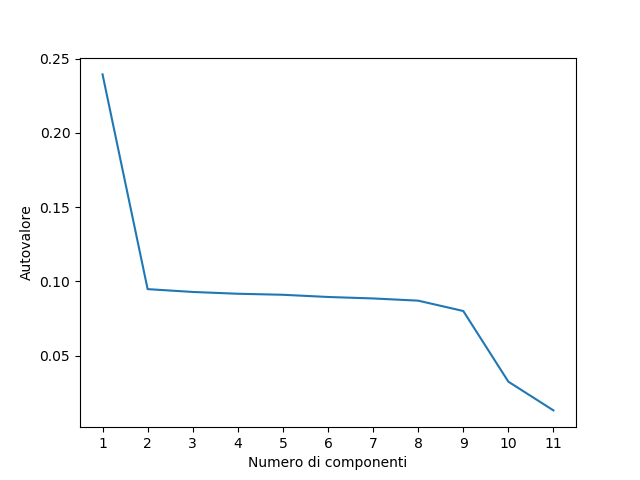
\includegraphics[width=0.4\textwidth]{img/scree_plot.png}
		\caption{scree plot del dataset Celiachion}
	\end{figure}

	La \emph{Figura 1} mostra lo scree-plot applicato al nostro dataset, che indicherebbe come migliore scelta un numero di componenti pari a 2 o 9, dal momento che è presente un "gomito netto" in corrispondenza di questi valori.


	\subsection{PCA}

	La \emph{Figura 2} mostra lo scatterplot 2D bidimensionale dopo aver ridotto il nostro dataset con due componenti per mezzo della tecnica di riduzione PCA.

	\begin{figure}[h]
		\centering
		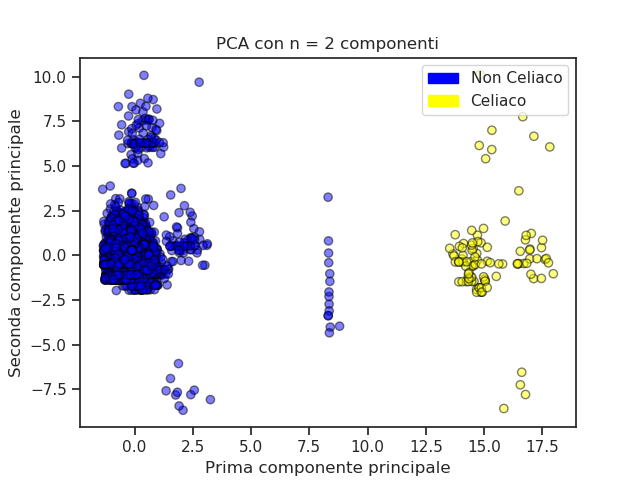
\includegraphics[width=0.4\textwidth]{img/PCA_2Dnc2.png}
		\caption{scatterplot 2D bidimensionale applicato su PCA}
	\end{figure}

	 L'uso dei colori - blu per la classe \emph{non celiaco} e giallo per la classe \emph{celiaco} - è un'ulteriore informazione che abbiamo voluto aggiungere per verificare la veridicità della separabilità di ciascuna tecnica di riduzione. \par
	 Dalla \emph{Figura 2} si evince che il PCA - con un numero di componenti principali pari a due - riesce a mantenere una buona separabilità dei data point, ad eccezione fatta per quelli centrali, i quali potrebbero essere facilmente fraintesi. \par

 	 Una situazione simile a quella di \emph{Figura 2} è evidente in \emph{Figura 3}, che mostra lo scatterplot 2D a seguito della riduzione della dimensionalità del dataset a tre componenti per mezzo della PCA.

	\begin{figure}[h]
		\centering
		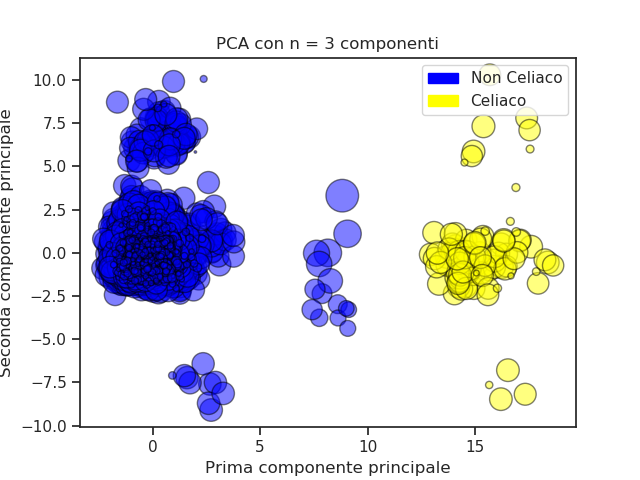
\includegraphics[width=0.4\textwidth]{img/PCA_2Dnc3.png}
		\caption{scatterplot 2D tridimensionale applicato su PCA}
	\end{figure}

	Ben evidente è la separabilità dei data point presenti nello scatterplot 3D interattivo, come visibile in \emph{Figura 4}.

	\begin{figure}[h]
		\centering
		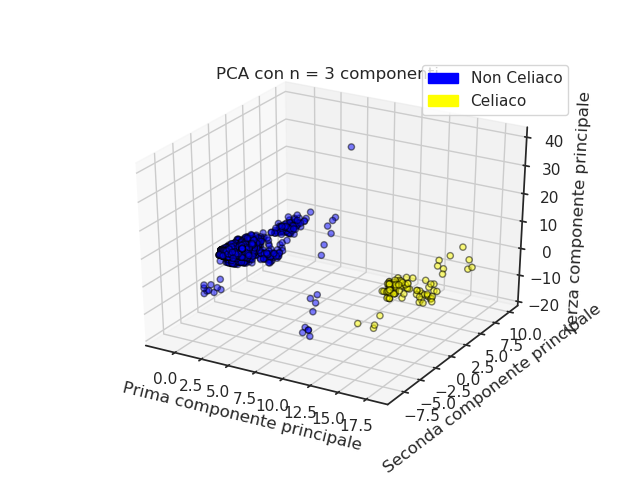
\includegraphics[width=0.4\textwidth]{img/PCA_i3D.png}
		\caption{scatterplot 3D interattivo applicato su PCA}
	\end{figure}

	Infine, la \emph{Figura 5} mostra il plot di Draftman applicato al dataset ridotto a 9 componenti per mezzo della tecnica PCA.

	\begin{figure}[h]
		\centering
		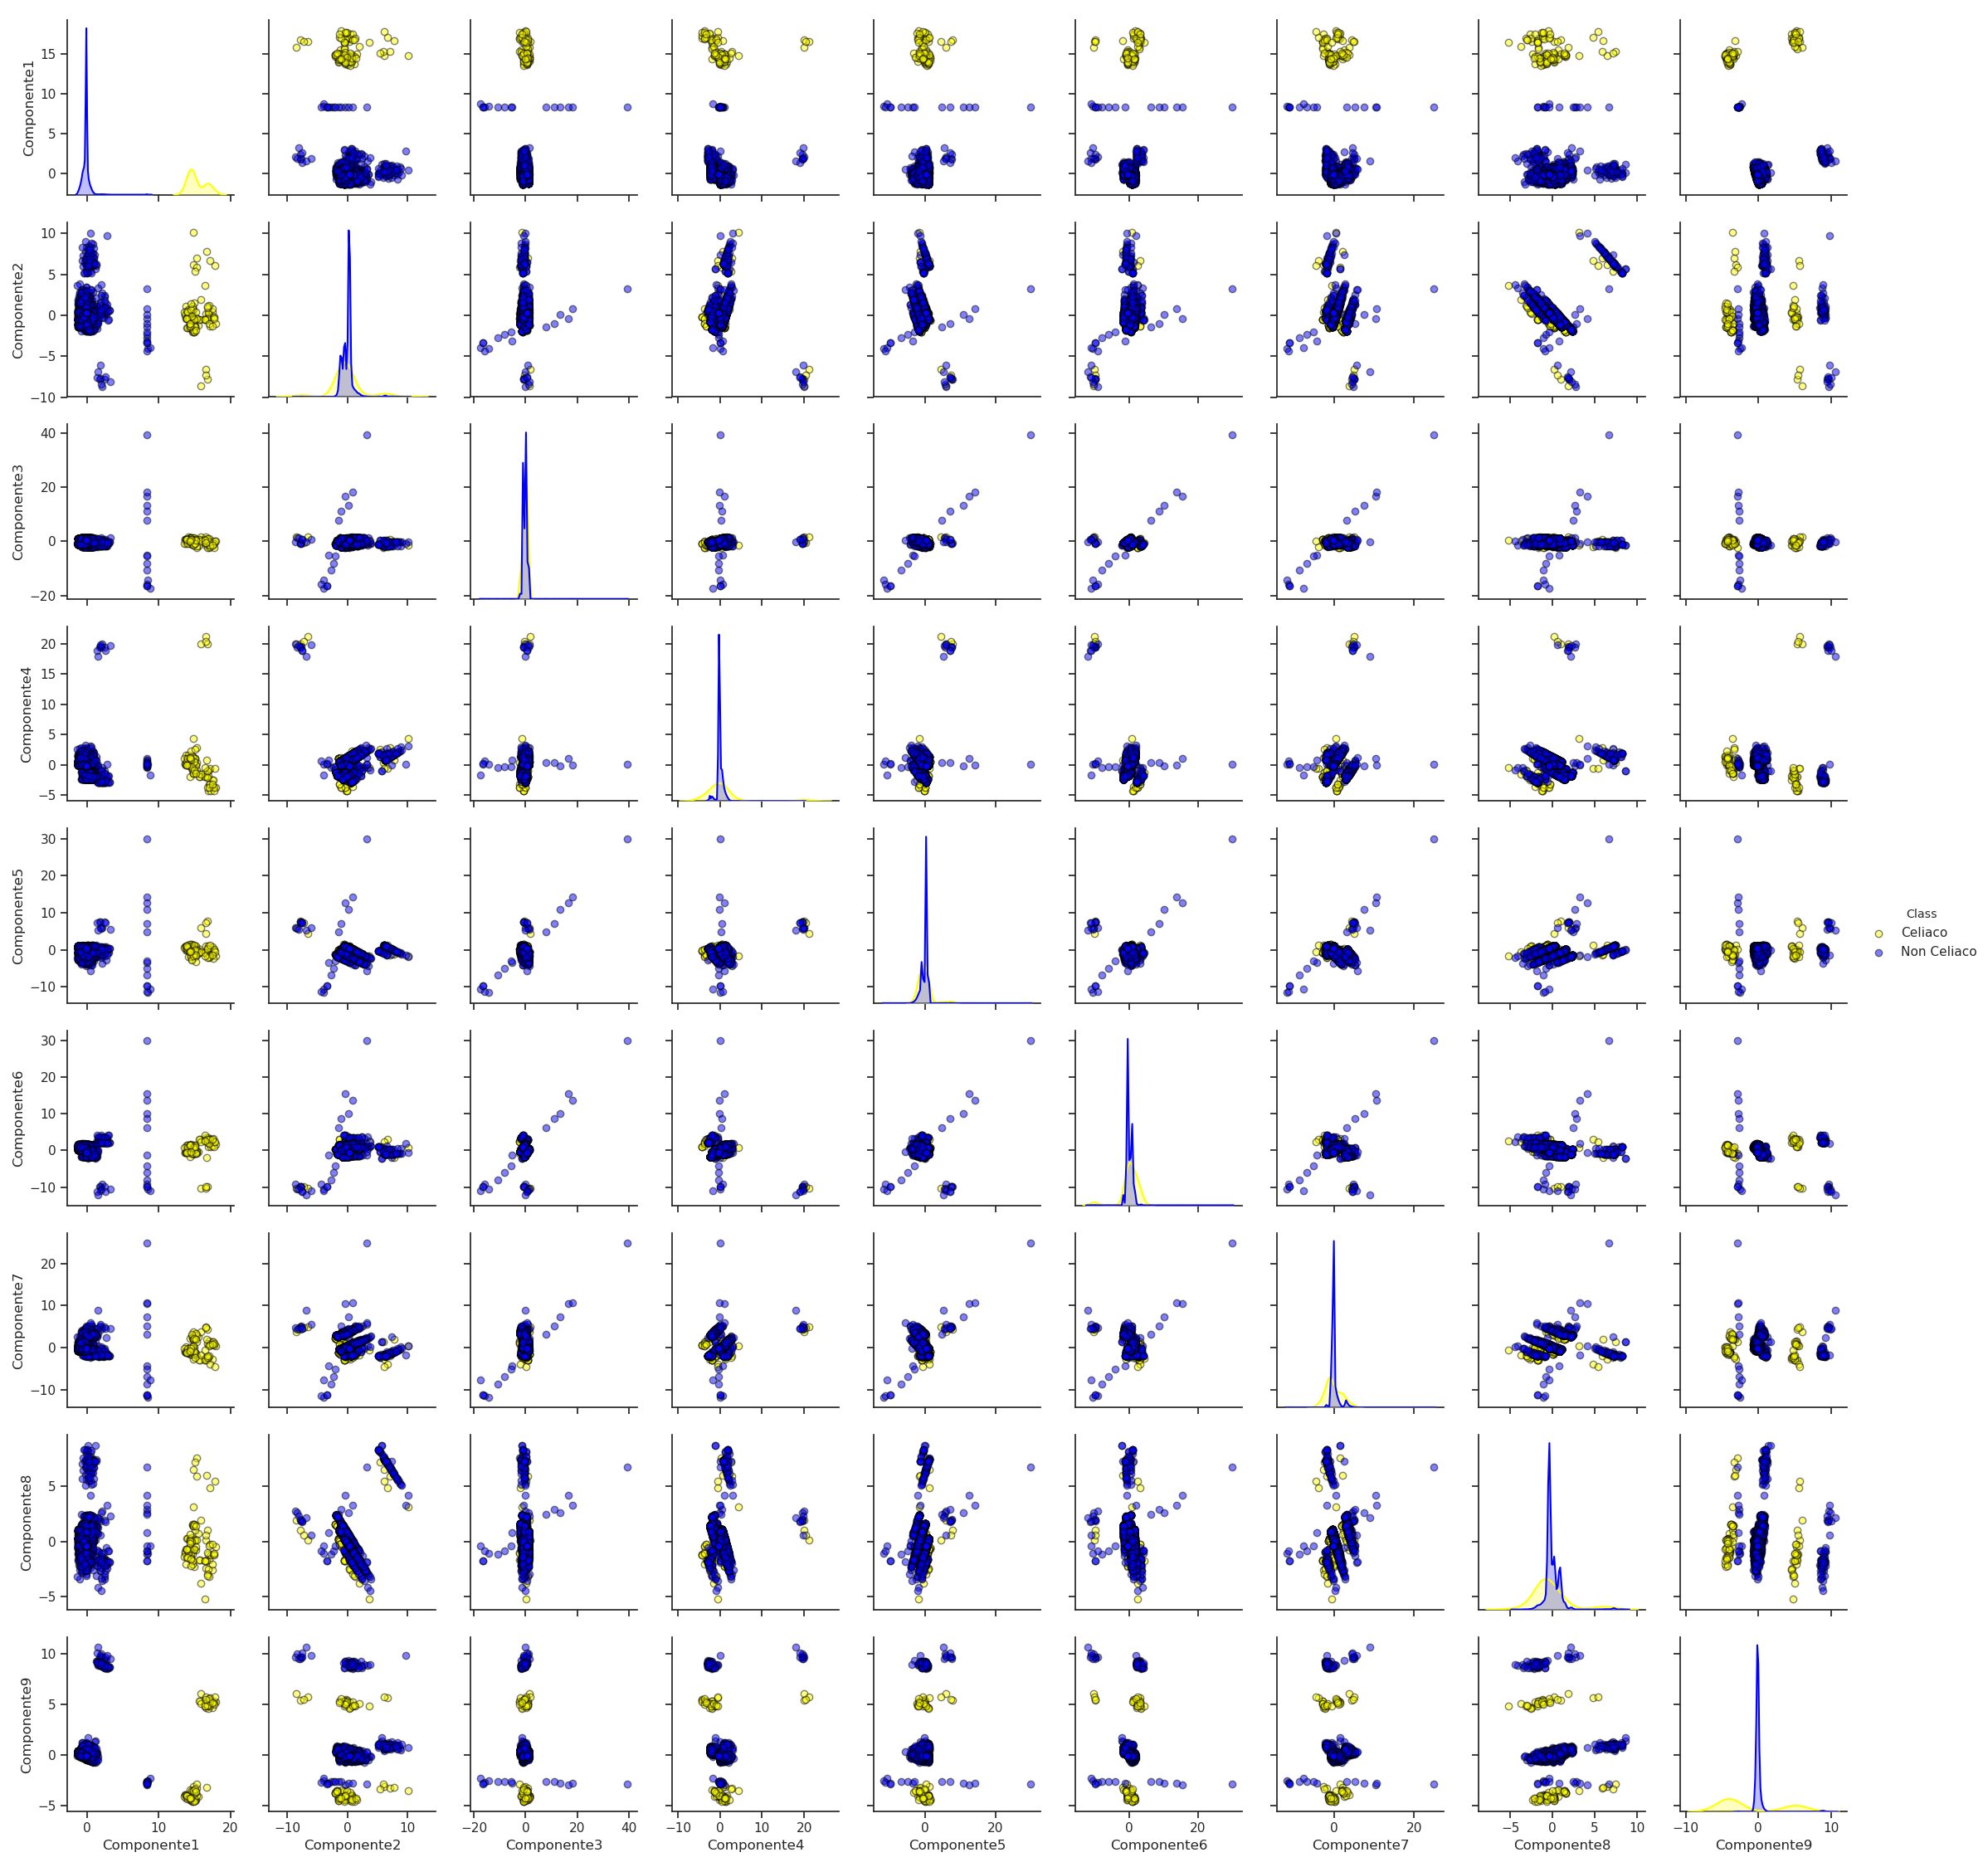
\includegraphics[width=0.4\textwidth]{img/PCA_SPLOM.png}
		\caption{plot di Draftman applicato su PCA}
	\end{figure}

	Da tale rappresentazione è possibile notare come la Componente 1, se messo in relazione con tutte le altre componenti della matrice, riesca a mantenere la migliore separabilità.


	\subsection{kernelPCA}

	In \emph{Figura 6} viene raffigurato lo scatterplot 2D bidimensionale a seguito della riduzione del dataset ridotto a due componenti per mezzo del kernelPCA.

	\begin{figure}[h]
		\centering
		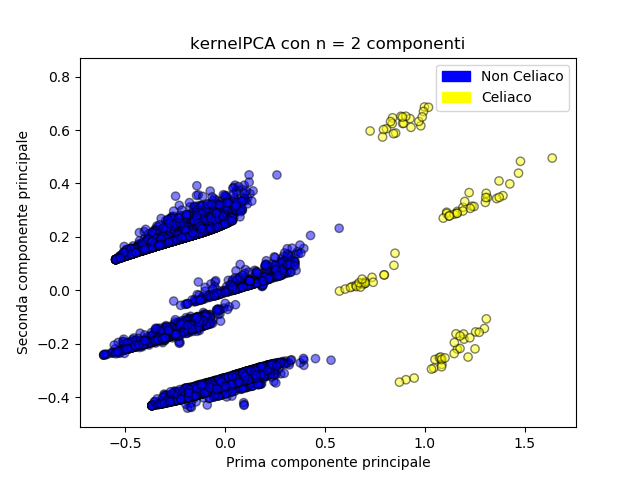
\includegraphics[width=0.4\textwidth]{img/kernelPCA_2Dnc2.png}
		\caption{scatterplot 2D bidimensionale applicato su kernelPCA}
	\end{figure}

	Da tale rappresentazione - anche se non in maniera netta, data la formazione di diverse agglomerazioni - si evince comunque una buona separabilità dei data point. \par

	La percezione di separabilità dei data point diminuisce drasticamente con il plot 2D tridimensionale, come ben visibile in \emph{Figura 7}.

	\begin{figure}[h]
		\centering
		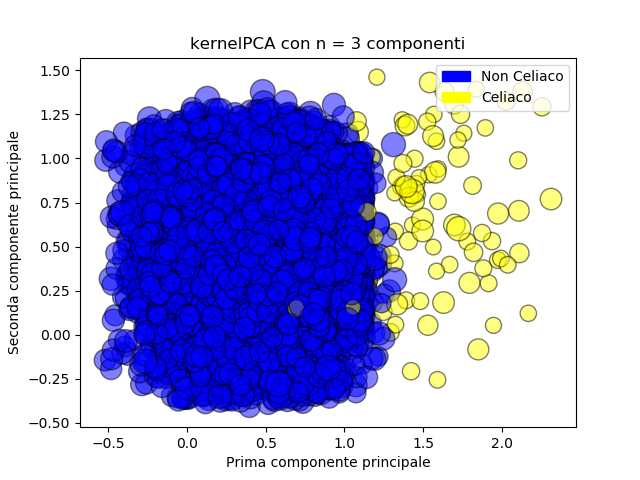
\includegraphics[width=0.4\textwidth]{img/kernelPCA_2Dnc3.png}
		\caption{scatterplot 2D tridimensionale applicato su kernelPCA}
	\end{figure}

	In \emph{Figura 8}, invece, é possibile notare come i data point siano ben distinti con una rappresentazione grafica 3D, risultando di fatto migliore delle precedenti per questa tecnica di riduzione.

	\begin{figure}[H]
		\centering
		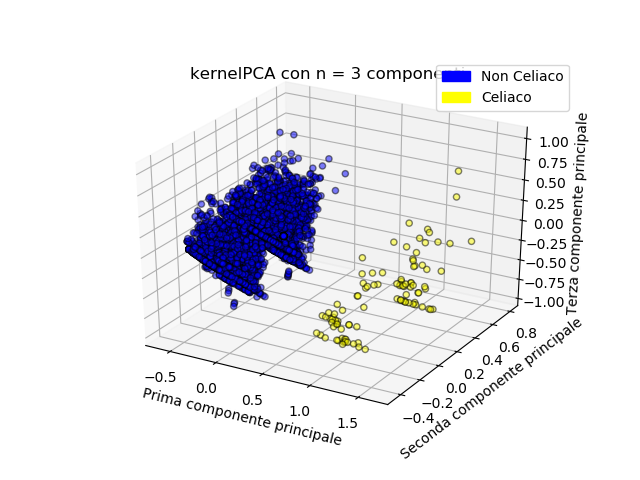
\includegraphics[width=0.4\textwidth]{img/kernelPCA_i3D.png}
		\caption{scatterplot 3D interattivo applicato su kernelPCA}
	\end{figure}

	Infine, la \emph{Figura 9} mostra il plot di Draftman applicato su kernelPCA per un numero di componenti pari a 9, del tutto simile al plot di Draftman applicato su PCA per lo stesso numero di componenti.

	\begin{figure}[h]
		\centering
		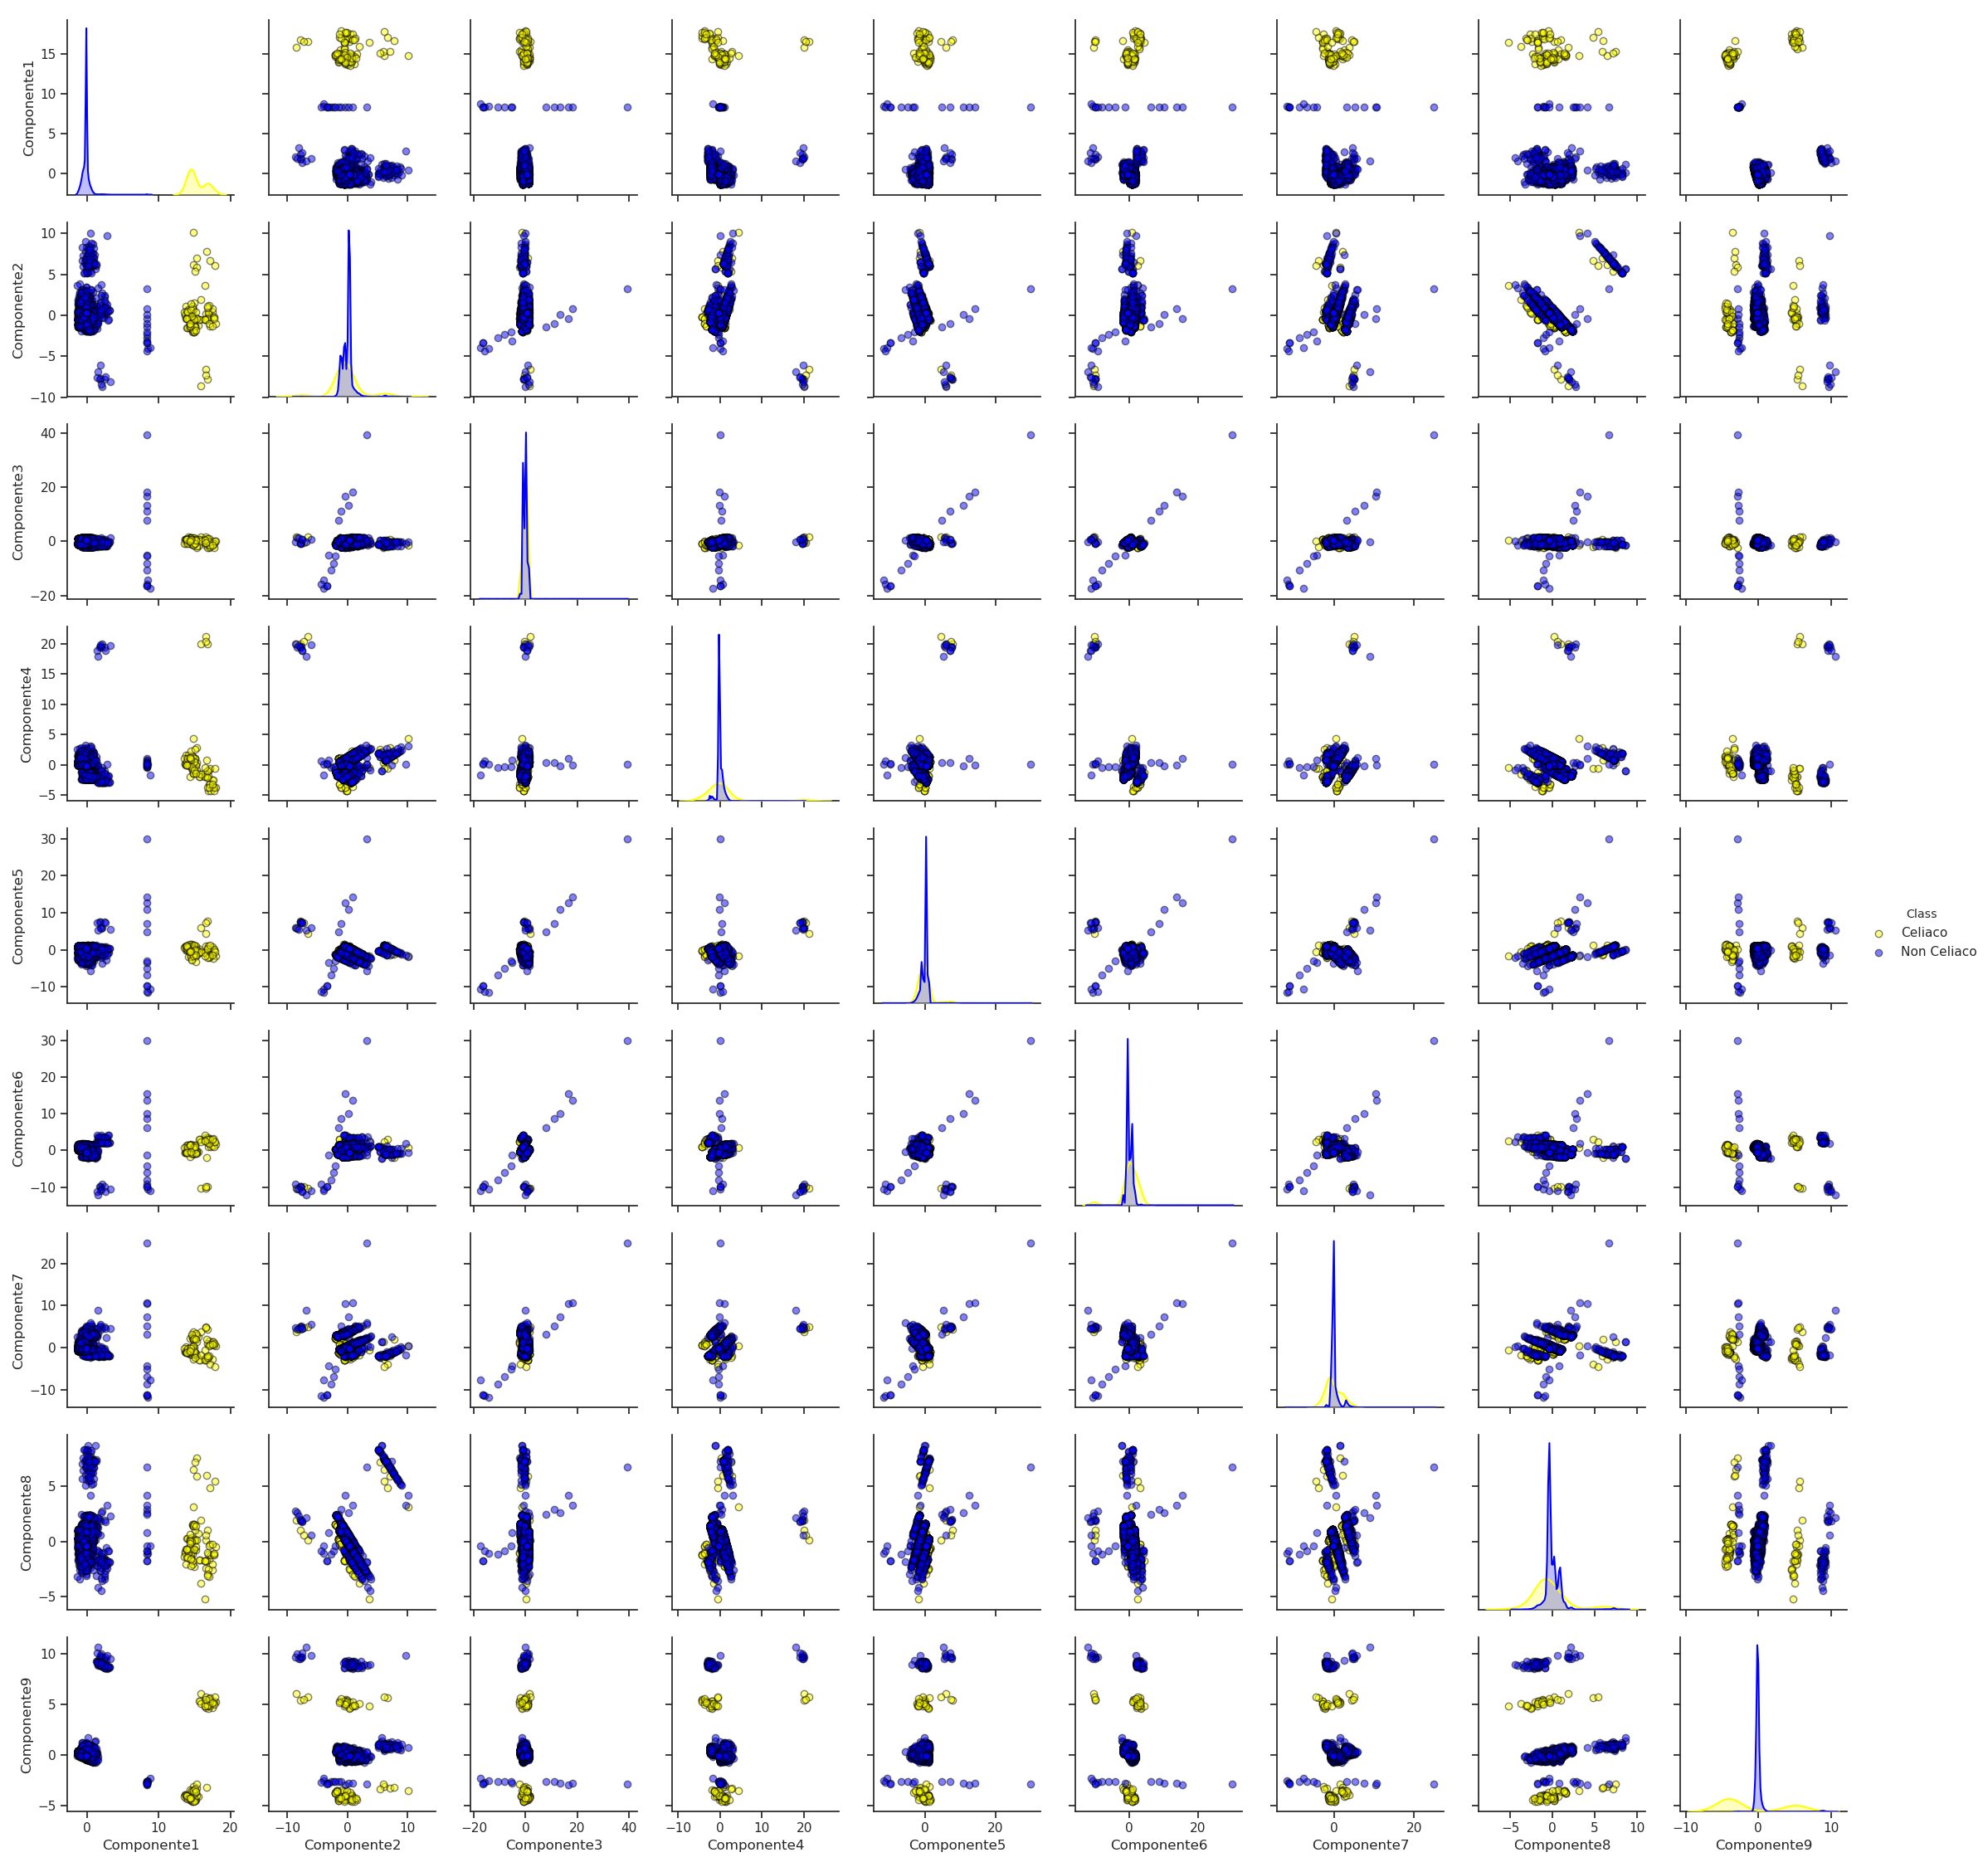
\includegraphics[width=0.4\textwidth]{img/kernelPCA_SPLOM.png}
		\caption{plot di Draftman applicato su kernelPCA}
	\end{figure}

	\subsection{MDS}

	La \emph{Figura 10} mostra lo scatterplot 2D bidimensionale del dataset ridotto a due componenti per mezzo del Multi-Dimensional Scaling (MDS).

	\begin{figure}[H]
		\centering
		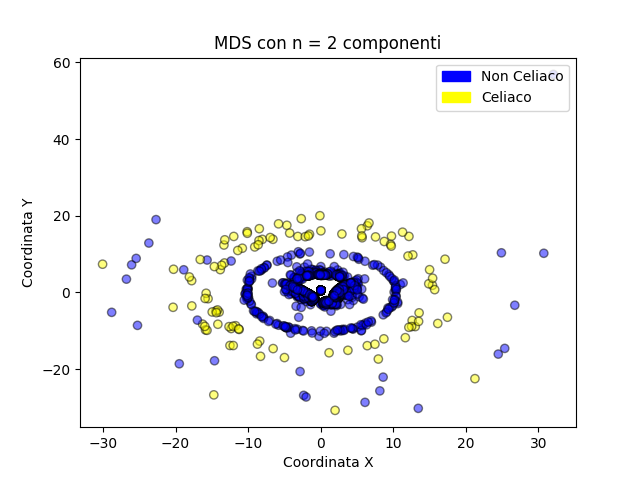
\includegraphics[width=0.5\textwidth]{img/MDS_2Dnc2.png}
		\caption{scatterplot 2D bidimensionale applicato su MDS}
	\end{figure}

	È possibile notare dallo scatterplot 2D bidimensionale come MDS riesca, nonostante i numerosi outliers, a distinguere i punti, seppur in maniera decisamente peggiore delle due tecniche di riduzione precedentemente descritte. Tuttavia, non si ha la medesima percezione applicando le altre tecniche di visualizzazione, come mostrato in \emph{Figura 11}, \emph{Figura 12} e \emph{Figura 13}.

	\begin{figure}[H]
		\centering
		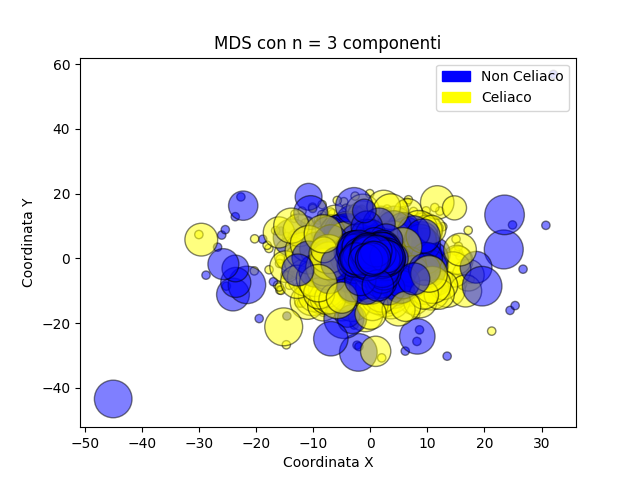
\includegraphics[width=0.5\textwidth]{img/MDS_2Dnc3.png}
		\caption{scatterplot 2D tridimensionale applicato su MDS}
	\end{figure}

	\begin{figure}[H]
		\centering
		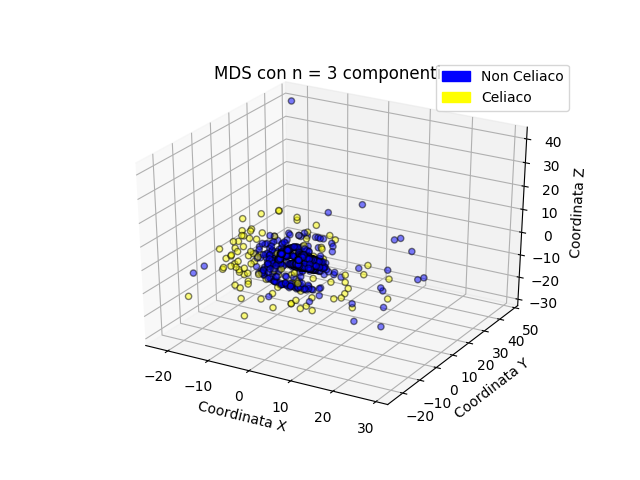
\includegraphics[width=0.5\textwidth]{img/MDS_i3D.png}
		\caption{scatterplot 3D interattivo applicato su MDS}
	\end{figure}

	\begin{figure}[H]
		\centering
		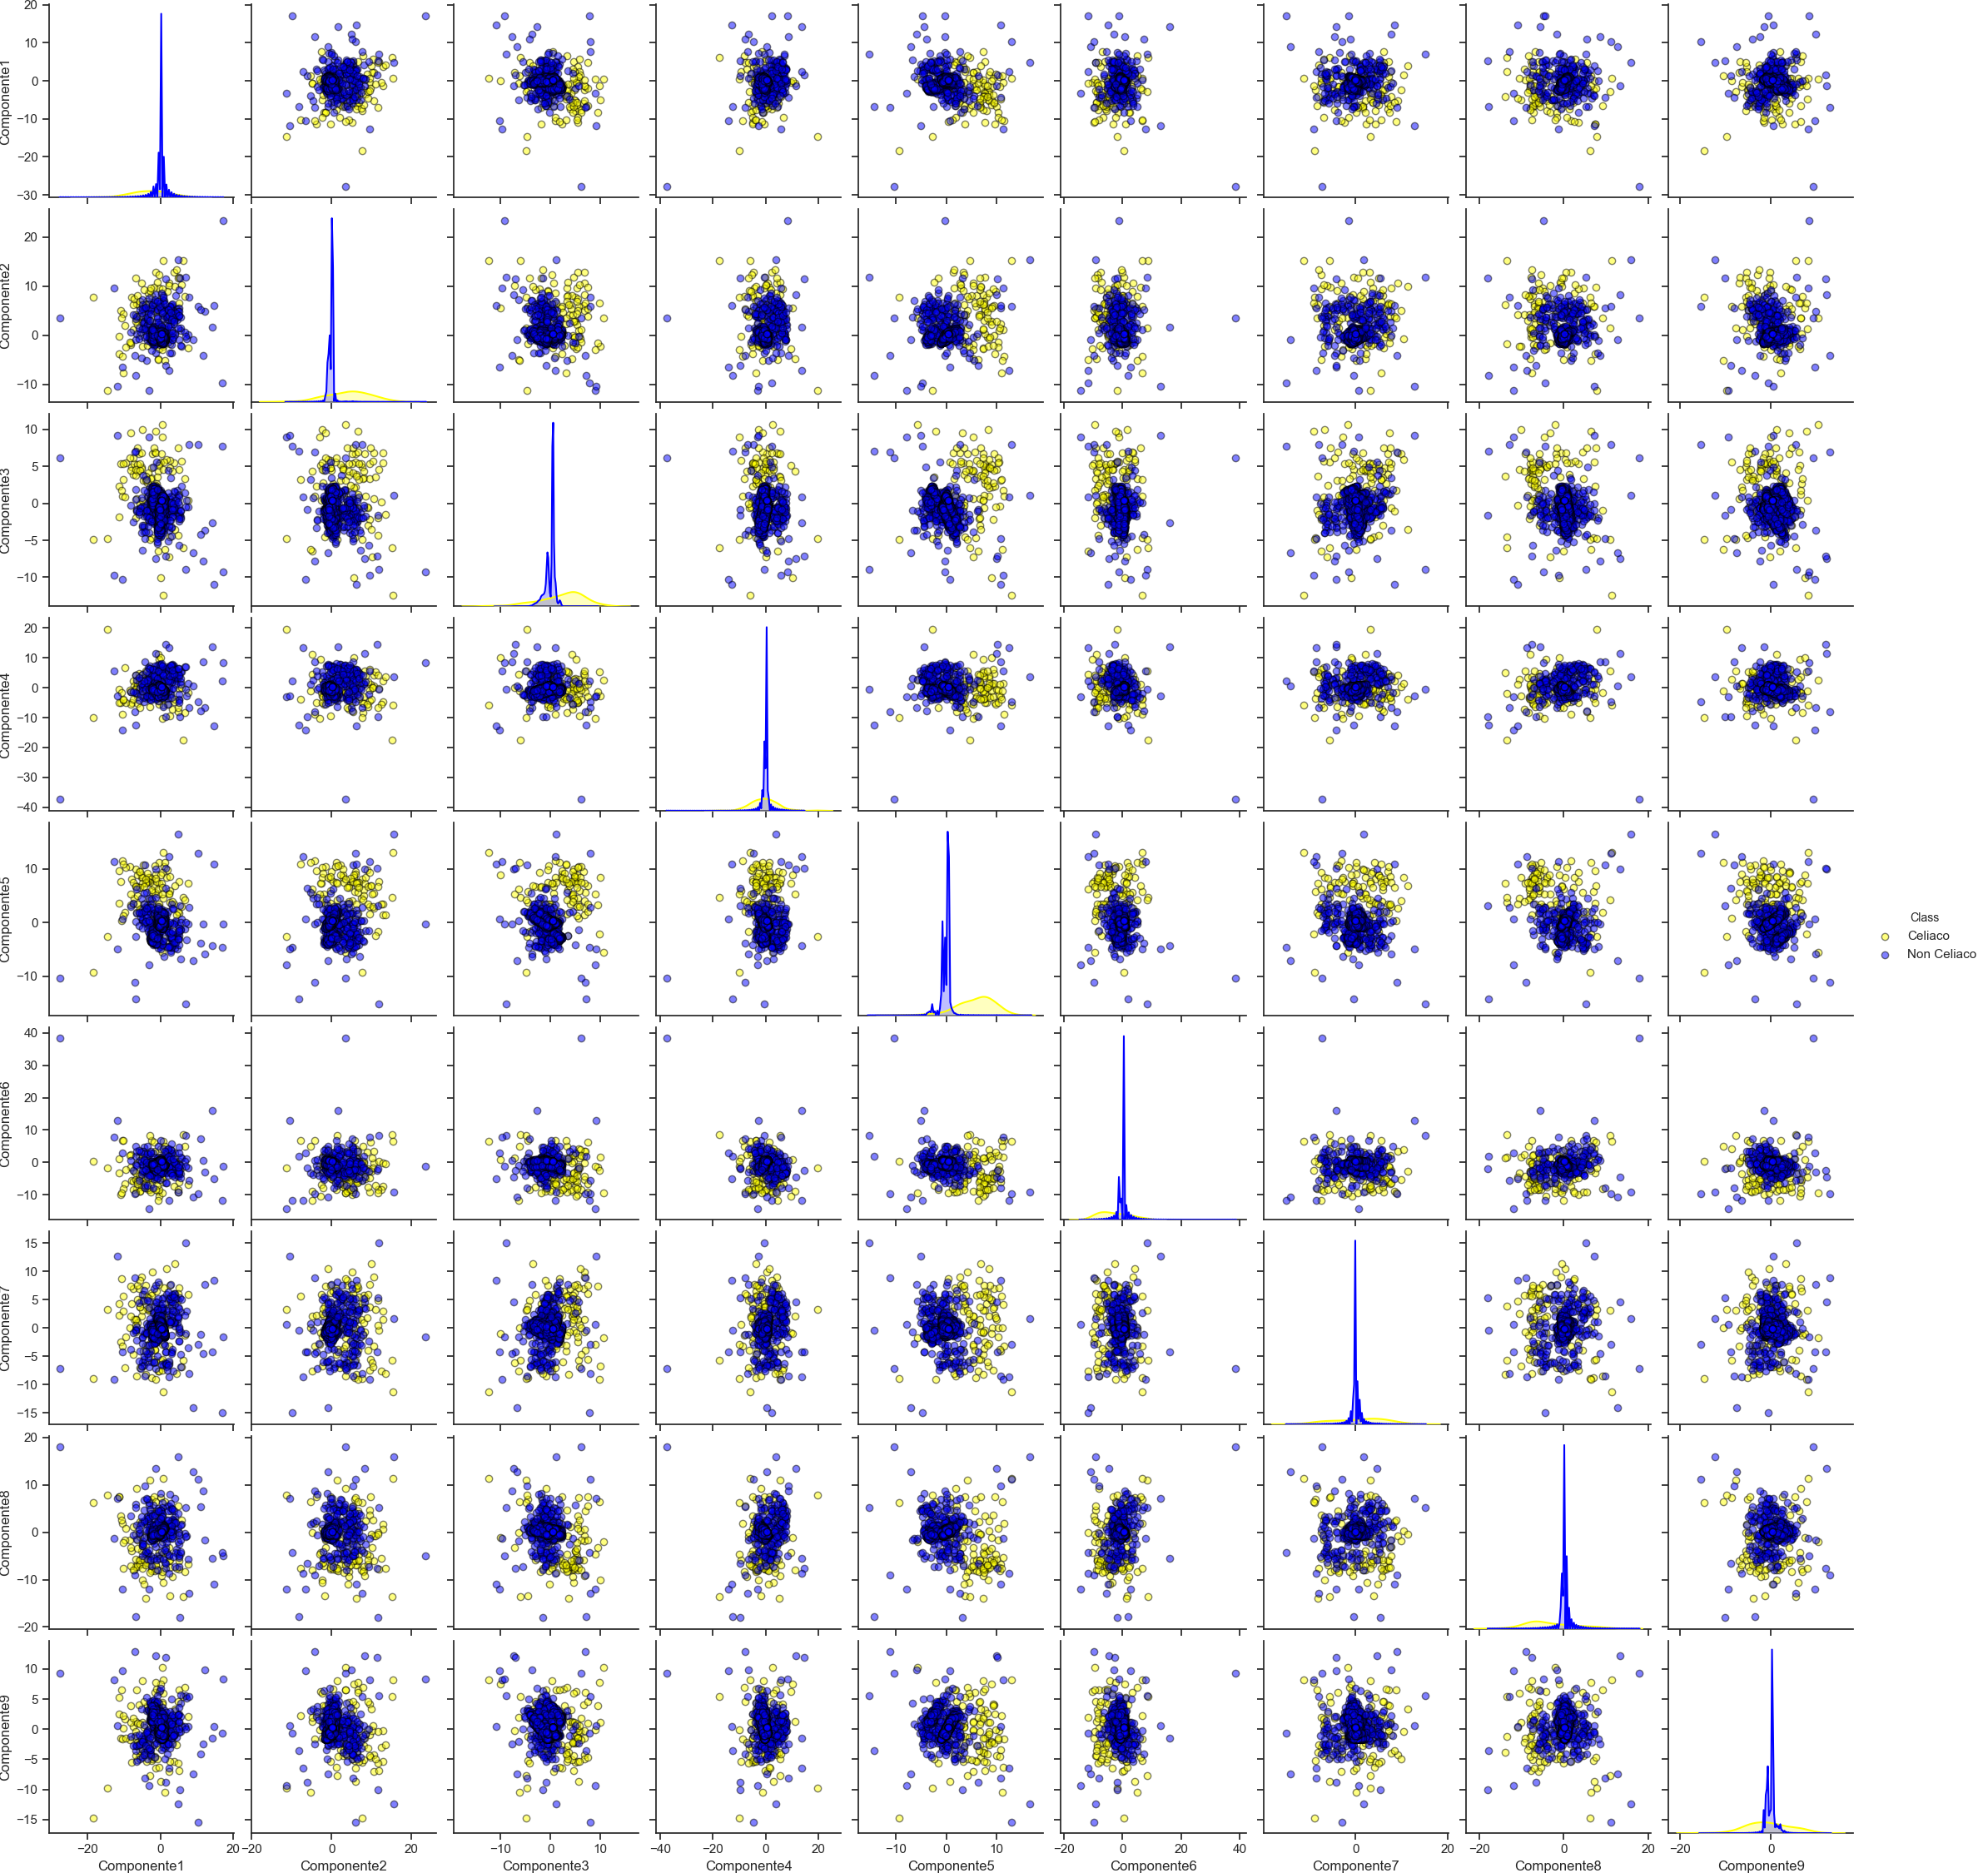
\includegraphics[width=0.5\textwidth]{img/MDS_SPLOM.png}
		\caption{plot di Draftman applicato su applicato su MDS}
	\end{figure}

    \subsection{t-SNE}

    L'ultima tecnica di riduzione applicata è il t-SNE, rivelatosi poco efficace per la separazione dei data point del dataset, come è possibile evincere in \emph{Figura 14}, \emph{Figura 15}, \emph{Figura 16} e \emph{Figura 17}.

	\begin{figure}[H]
		\centering
		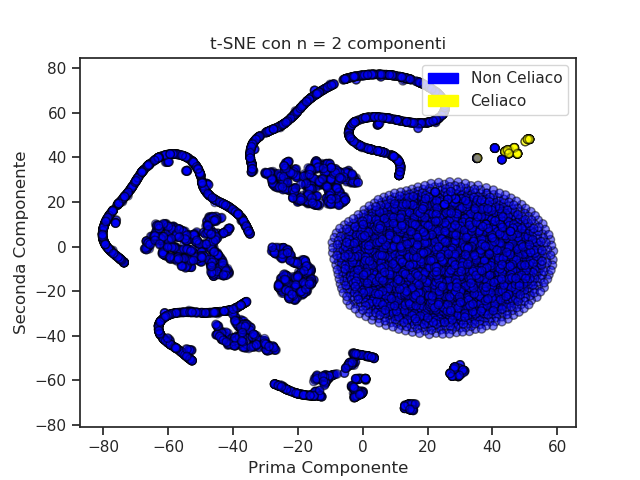
\includegraphics[width=0.4\textwidth]{img/tSNE_2Dnc2.png}
		\caption{scatterplot 2D bidimensionale applicato su t-SNE}
	\end{figure}

	\begin{figure}[H]
		\centering
		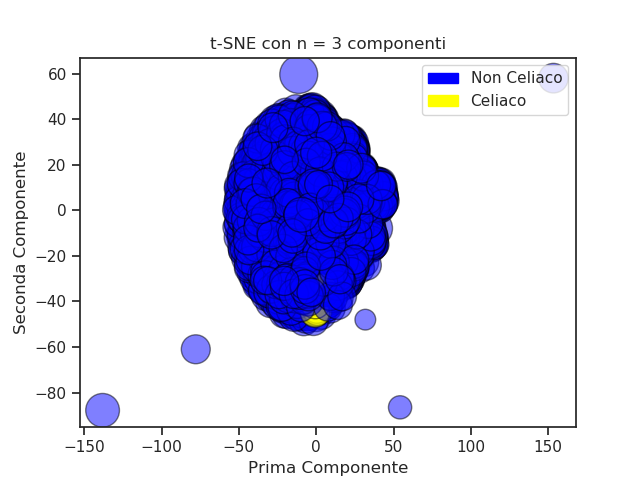
\includegraphics[width=0.4\textwidth]{img/tSNE_2Dnc3.png}
		\caption{scatterplot 2D tridimensionale applicato su t-SNE}
	\end{figure}

	\begin{figure}[H]
		\centering
		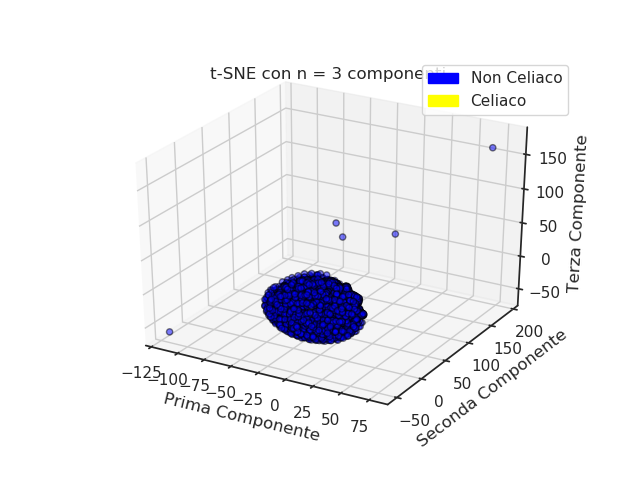
\includegraphics[width=0.4\textwidth]{img/tSNE_i3D.png}
		\caption{scatterplot 3D interattivo applicato su t-SNE}
	\end{figure}

	\begin{figure}[H]
		\centering
		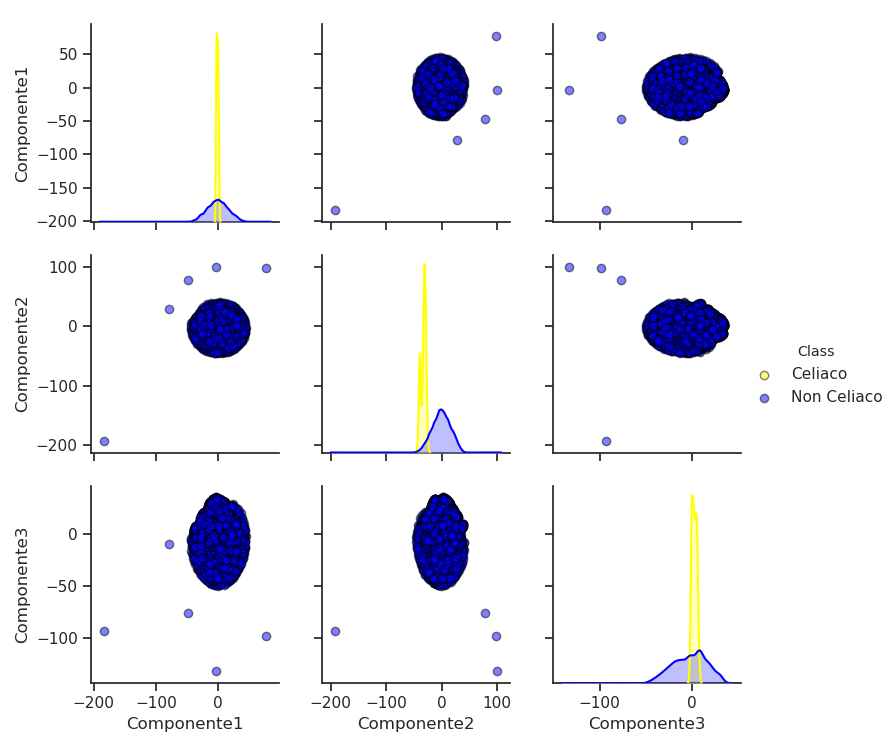
\includegraphics[width=0.4\textwidth]{img/tSNE_SPLOM.png}
		\caption{plot di Draftman applicato su t-SNE}
	\end{figure}


\section{Alberi decisionali}
In machine learing, un albero decisionale è la rappresentazione di un modello predittivo progettato al fine di classificare le istanze di grandi quantità di dati (per questo motivo viene anche chiamato albero di classificazione), contenente solamente strutture selettive.\par
In un albero decisionale:
\begin{itemize}
	\item ogni nodo interno effettua un test su un attributo. Questo test può risultare dunque vero o falso
	\item i nodi interni sono collegati attraverso rami corrispondenti ai risultati dei test
	\item ogni foglia rappresenta il valore predetto
	\item ad ogni nodo interno viene spesso associato un \emph{tasso d'errore}, un \emph{indice di Gini} oppure una \emph{variazione di entropia}
\end{itemize}
Allora, dato un albero decisionale generato addestrando il modello predittivo tramite un training set, per classificare una istanza è necessario e sufficiente esaminare l'unico cammino radice-foglia compiuto da tale istanza.\par
In particolare, in questo studio, ad ogni nodo interno dell'albero è stato associato l'\emph{indice di Gini}, indice di eterogeneità per variabili qualitative. Più precisamente, l'indice di Gini offre una misura della eterogeneità di una distribuzione statistica a partire dai valori delle frequenze relative associate alle \emph{k} modalità di una generica variabile \emph{X}.

\subsection{Classificazione "nome dataset" non ridotto}
In \emph{Figura 18} viene mostrato l'albero decisionale generato a partire dal dataset non ridotto. In particolare, in questo albero, il 98\% dei pazienti viene classificato attraverso il percorso radice-foglia più a sinistra.

\begin{figure}[H]
	\centering
	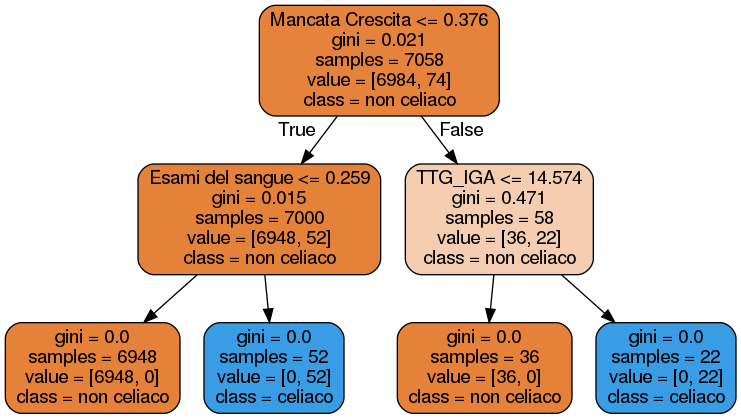
\includegraphics[width=0.4\textwidth]{img/decision_tree.png}
	\caption{albero decisionale prodotto a partire dal dataset non ridotto.}
\end{figure}

A partire da questo albero, è stato possibile successivamente generare anche un \emph{treemap}, come mostrato in \emph{Figura 19}, utile per visualizzare graficamente i percorsi radice-foglie più rilevanti coinvolti nella classificazione.
\begin{figure}[H]
	\centering
	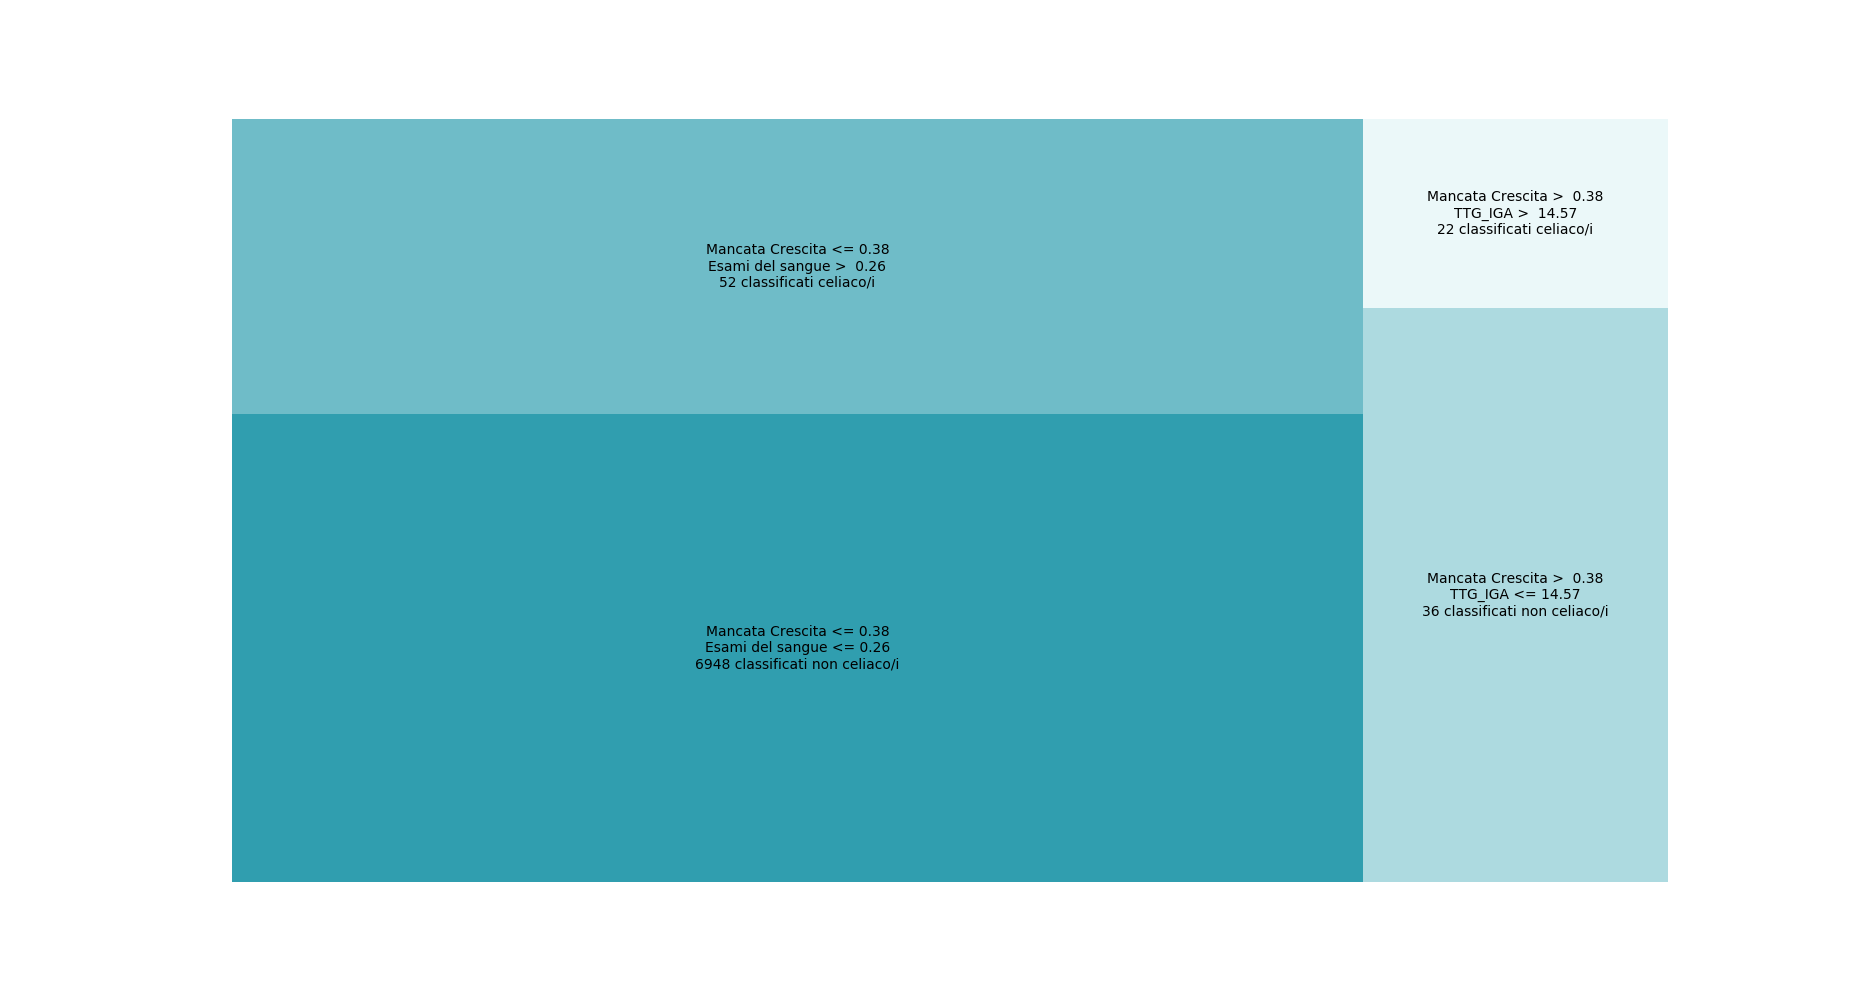
\includegraphics[width=0.45\textwidth]{img/treemap.png}
	\caption{treemap corrispondente all'albero decisionale. Evidenzia quale siano le foglie più rilevanti.}
\end{figure}

\subsection{Classificazione "nome dataset" ridotto}
In \emph{Figura 20} viene mostrato invece l'albero decisionale generato a partire dal dataset ridotto a 3 componenti tramite la tecnica PCA.
\begin{figure}[H]
	\centering
	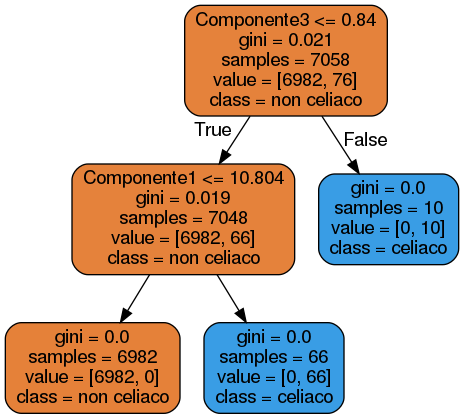
\includegraphics[width=0.25\textwidth]{img/decision_tree_PCA.png}
	\caption{albero decisionale prodotto per il dataset ridotto tramite la tecnica PCA.}
\end{figure}

Di seguito vengono mostrati anche in \emph{Figura 21}, \emph{Figura 22} e \emph{Figura 23}, gli alberi decisionali rispettivamente per il dataset ridotto a 3 componenti mediante le tecniche di kernel PCA, MDS e t-SNE.
\begin{figure}[H]
	\centering
	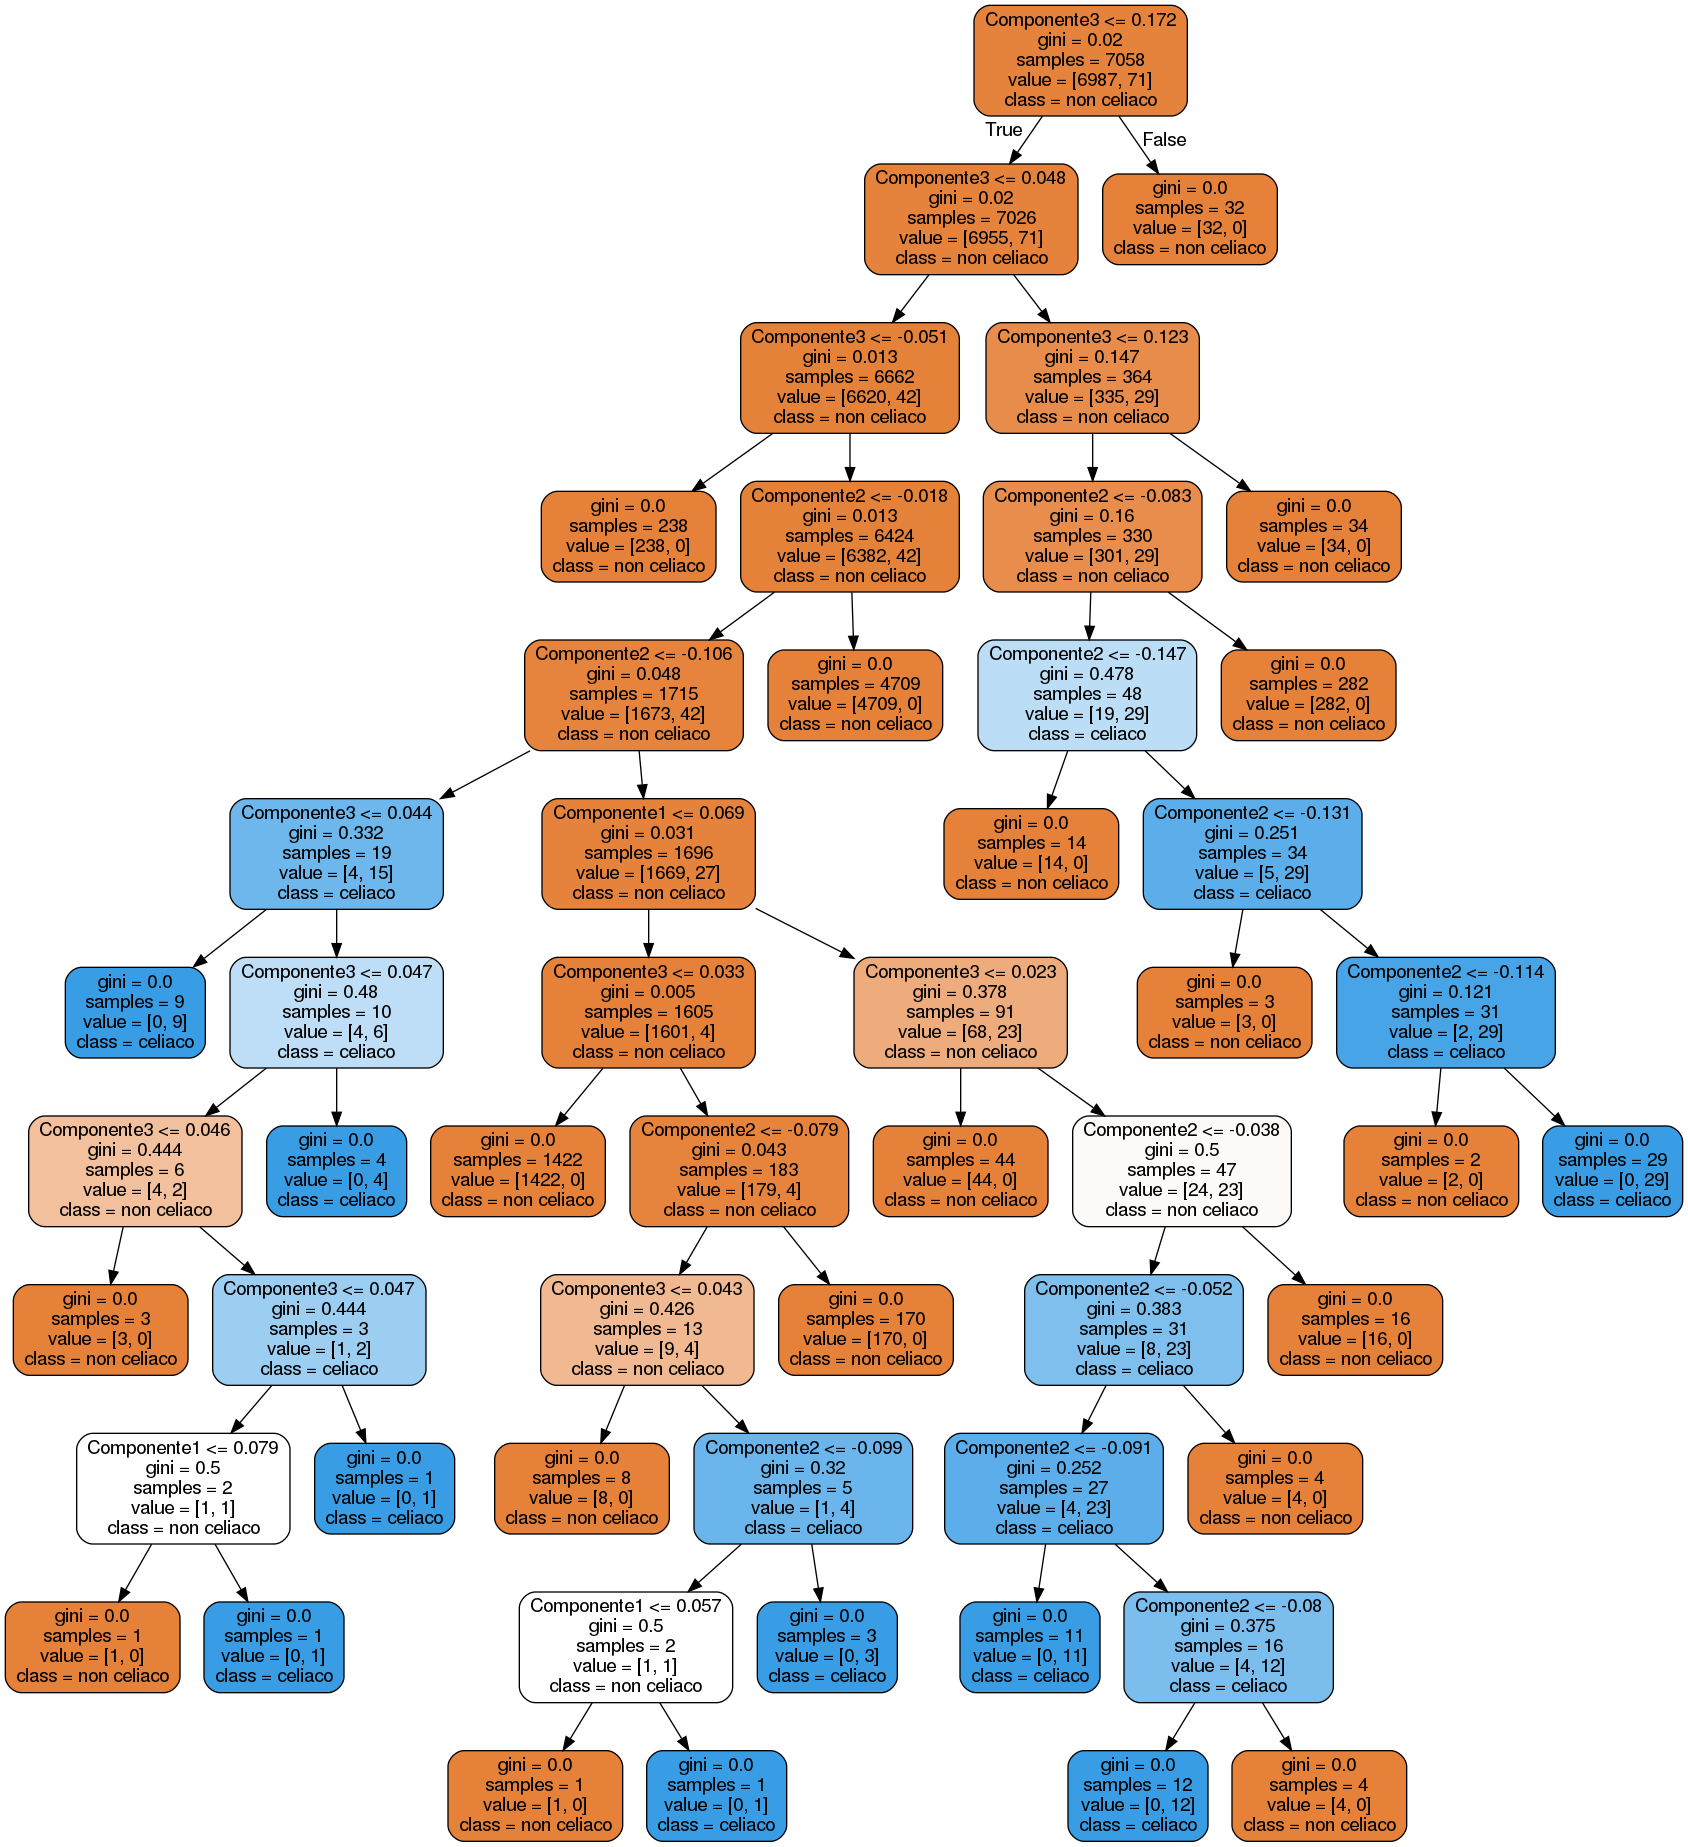
\includegraphics[width=0.4\textwidth]{img/decision_tree_kernelPCA.png}
	\caption{albero decisionale prodotto per il dataset ridotto tramite la tecnica kernel PCA.}
\end{figure}
\begin{figure}[H]
	\centering
	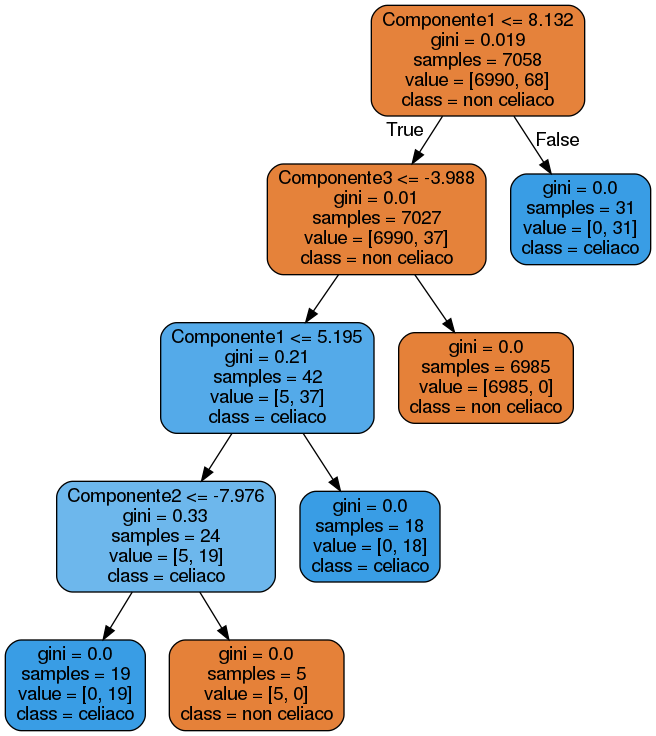
\includegraphics[width=0.3\textwidth]{img/decision_tree_MDS.png}
	\caption{albero decisionale prodotto per il dataset ridotto tramite la tecnica MDS.}
\end{figure}
\begin{figure}[H]
	\centering
	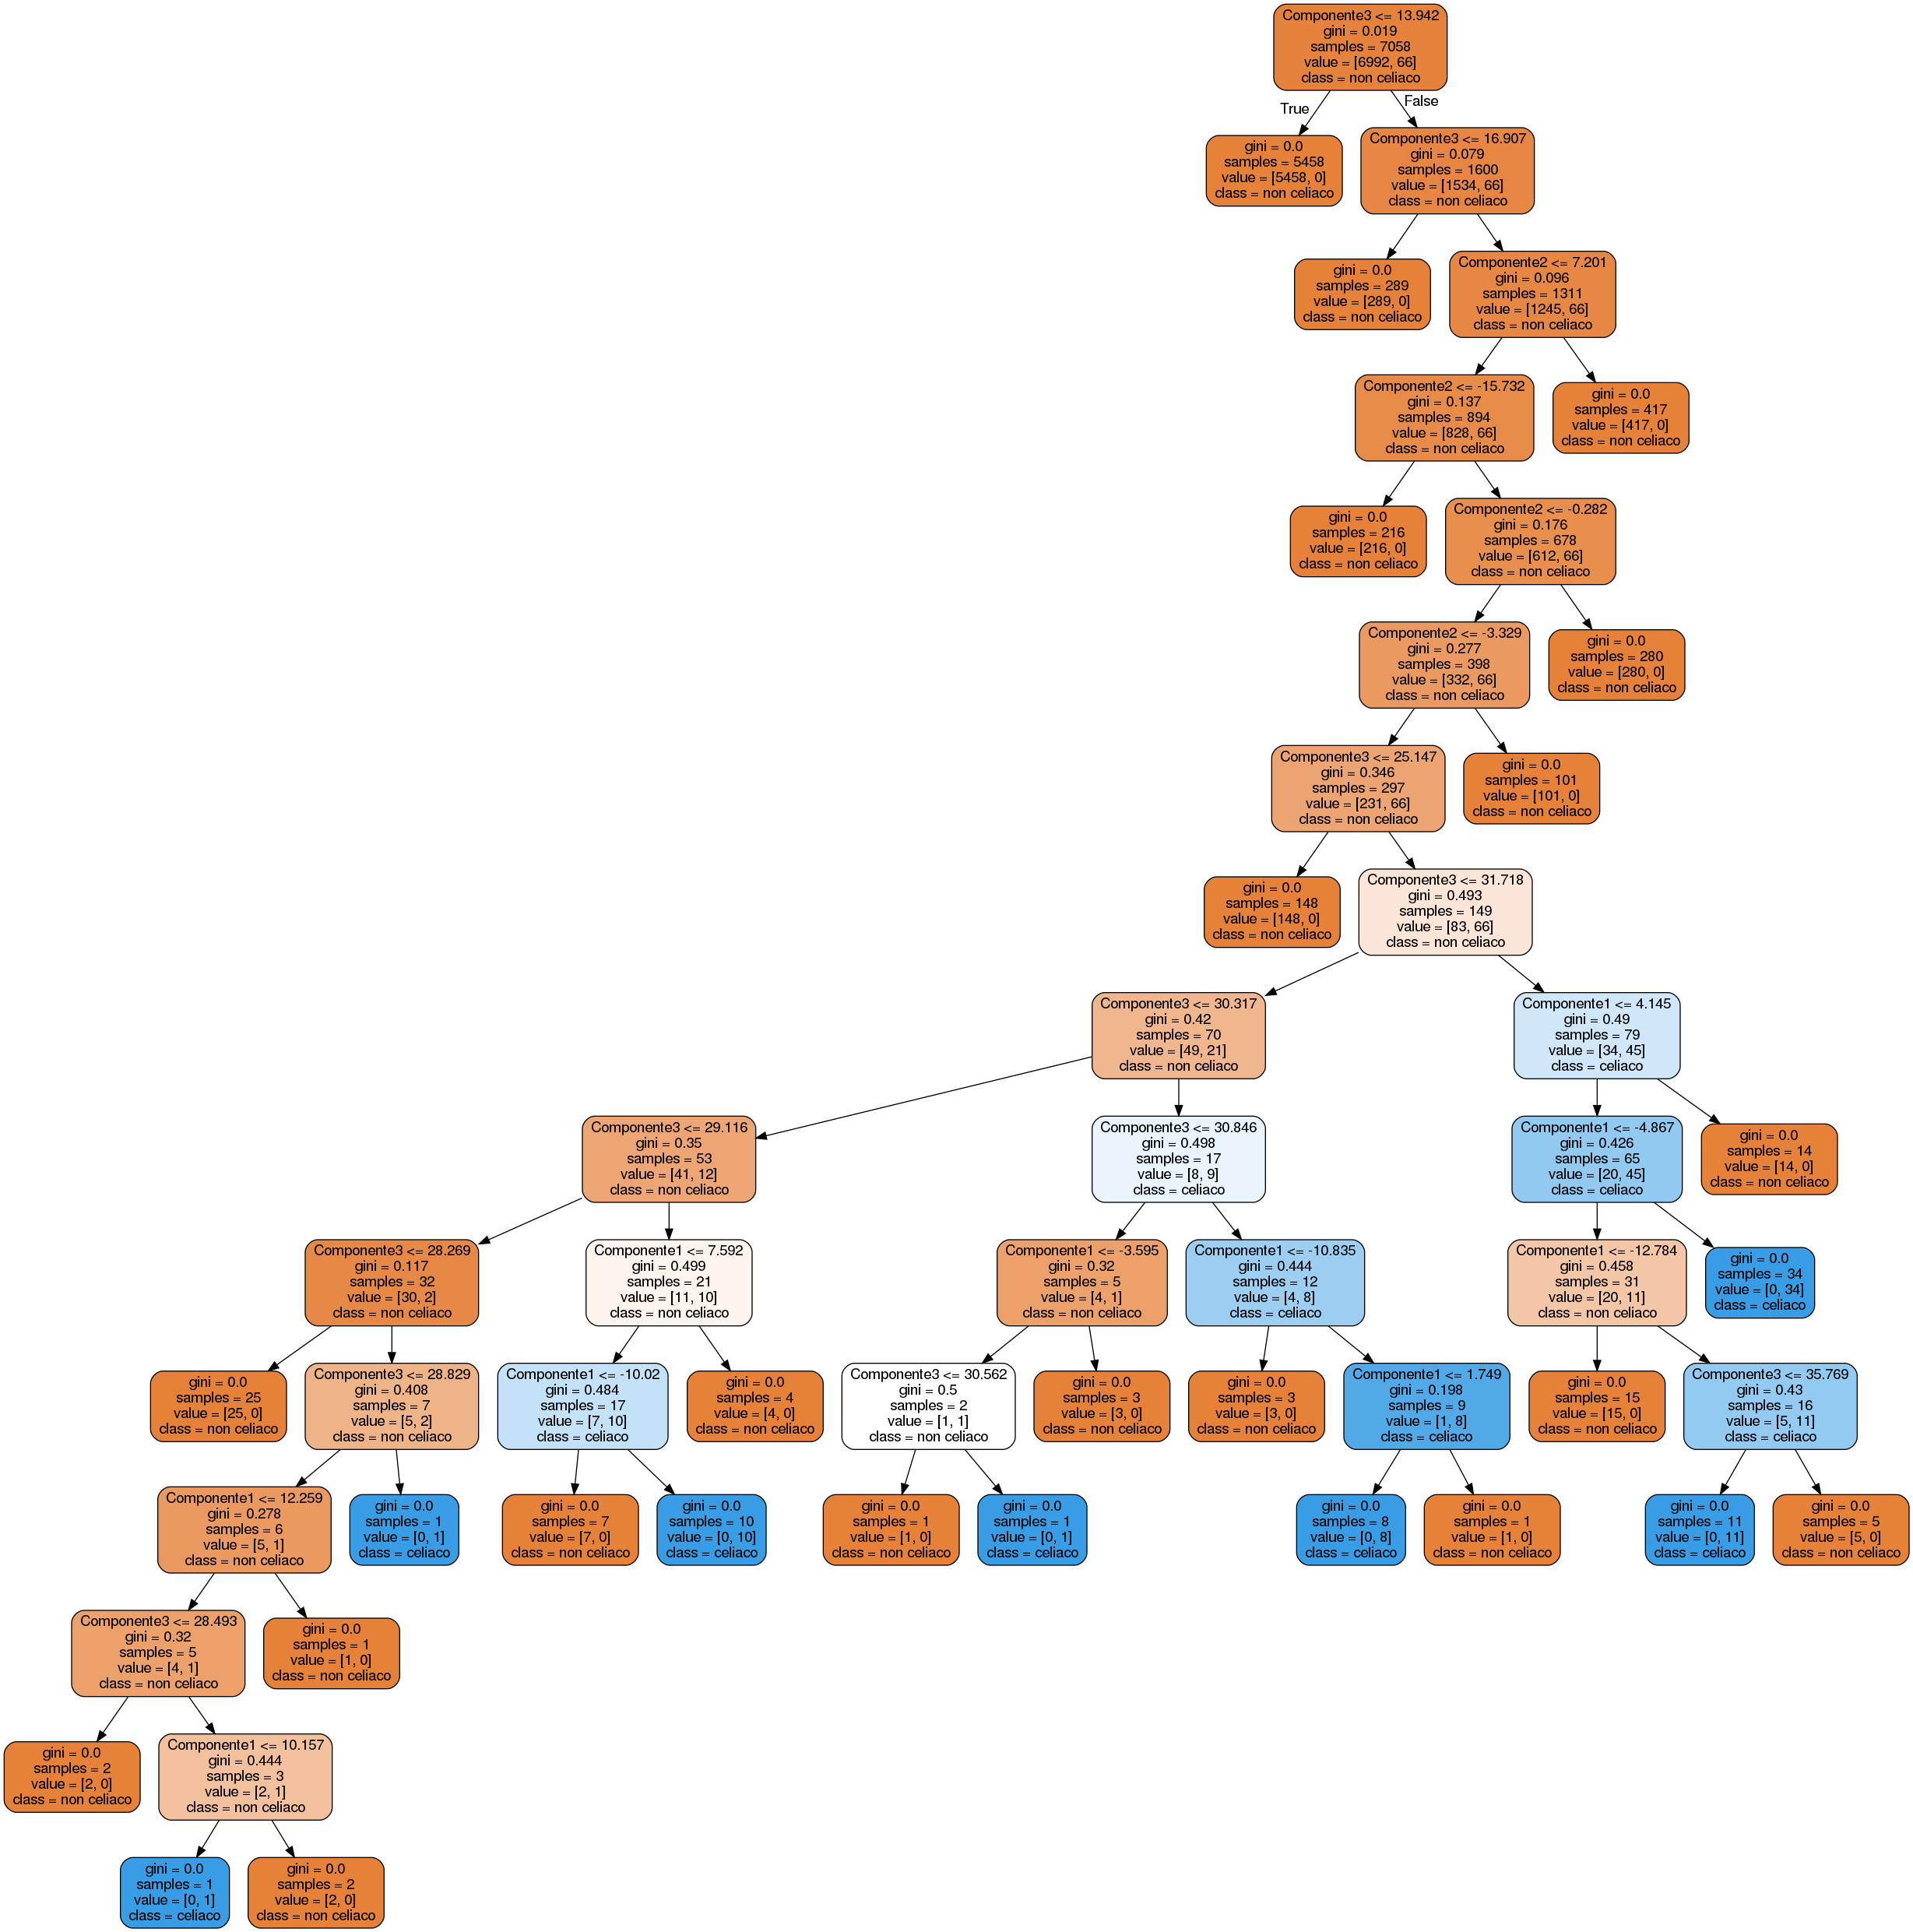
\includegraphics[width=0.4\textwidth]{img/decision_tree_tSNE.png}
	\caption{albero decisionale prodotto per il dataset ridotto tramite la tecnica t-SNE.}
\end{figure}

\section{Conclusioni}
Le tecniche di riduzione dimensionale più efficaci tra quelle discusse in questo studio sono risultate essere la PCA e la kernelPCA, come dimostrato in \emph{Figura 2}, \emph{Figura 3}, \emph{Figura 4}, \emph{Figura 5} per la PCA, e in \emph{Figura 6}, in \emph{Figura 8} e in \emph{Figura 9} per il kernelPCA. \par

In particolare, per la PCA è stato condotto un ulteriore studio volto ad interpretare le componenti. Come mostrato in \emph{Figura 24}, la prima componente principale è fortemente influenzata dai parametri \emph{Esami del sangue}, \emph{TTG IGA} e \emph{POCT}, mentre la seconda componente principale dai parametri \emph{IGA totali} e \emph{Madre Celiaca}.

\begin{figure}[H]
	\centering
	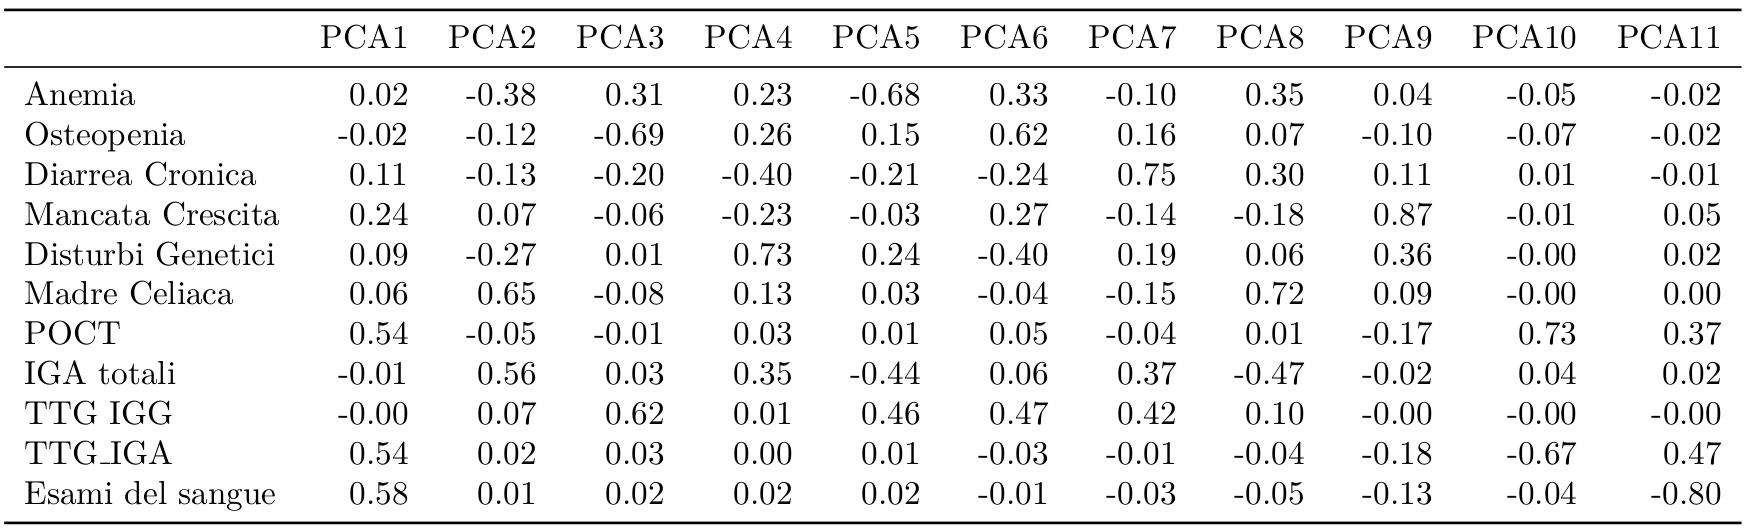
\includegraphics[width=0.45\textwidth]{img/PCA_components_interpretation.png}
	\caption{Interpretazione delle componenti del dataset "nomedataset" per la tecnica di riduzione PCA}
\end{figure}

Inoltre, a seguito dei risultati ottenuti in \emph{Figura 2} e \emph{Figura 24}, è stata condotta una ricerca approfondita per l'individuazione dei data point allineati appartenenti al cluster centrale di \emph{Figura 2}. La \emph{Figura 25} mostra la lista dei pazienti corrispondenti a quei punti. È stato, infatti, interessante notare come una combinazione di valori di \emph{Esami del sangue=0.0}, \emph{TTG IGA=NaN} e \emph{POCT=2.0} possa essere possibile causa di fraintendimento per la diagnosi della celiachia in un paziente.

\begin{figure}[H]
	\centering
	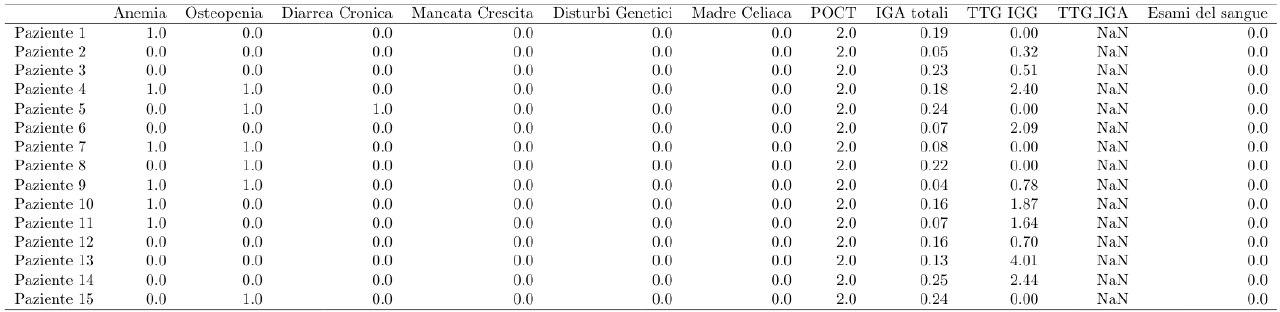
\includegraphics[width=0.45\textwidth]{img/pazientiFiltrati.png}
	\caption{lista dei pazienti corrispondenti ai punti allineati del cluster centrale di \emph{Figura 2}}
\end{figure}

Tutti gli alberi decisionali generati sono risultati molto efficaci nel classificare i pazienti virtuali. Infatti, l'albero decisionale per il dataset:
\begin{itemize}
	\item non ridotto è accurato al 100\%
	\item ridotto tramite PCA è accurato al 100\%
	\item ridotto tramite kernelPCA è accurato al 99\%
	\item ridotto tramite MDS è accurato al 99\%
	\item ridotto tramite t-SNE è accurato al 99\%
\end{itemize}
Quindi, l'albero decisionale corrispondente alla tecnica PCA risulta il più efficace, oltre che il più semplice in termini di profondità. Di contro, gli alberi decisionali risultanti dalle applicazioni delle tecniche kernelPCA e t-SNE risultano i più complessi.
\end{document}
